\chapter{CCD-based Multispectral Frequency-domain DOT: Instrumentation, Pre-clinical and Clinical Results}
\label{Chap:4_Gen3}
\section{Introduction}
Our group at Penn has played a leading role developing Diffuse Optical Tomography (DOT) for breast imaging and, more generally, translating DOT techniques to the clinic \cite{Corlu2003,Culver2003a,Holboke2000,Ntziachristos1999,Ntziachristos2001,Ntziachristos2000,Ntziachristos2002,OLeary1996,Zhu1999}. My work improves on this research by addressing critical limitations of the early DOT imagers, that last of which I will refer to herein as the Gen2 instrument. These limitations were ascertained through various clinical studies \cite{Culver2003,Corlu2003,Corlu2005,Choe2005a,Corlu2007,Choe2009}.

My DOT imager, which I will refer to herein as the Gen3 instrument, introduced significant new capabilities for improved breast-DOT: 1) A multispectral \textit{frequency-domain} mode of operation in the transmission geometry that employs heterodyne detection; 2) the world's \textit{largest} clinical source-detector \textit{data set} to facilitate high-fidelity 3D DOT reconstruction; 3) multiple channels for \textit{real-time normalization} of instrument phase and amplitude shifts/drifts; and  4) a projection-camera \textit{profilometry system} for defining breast boundaries and thereby facilitating improved breast segmentation; 5) an improved clinical \textit{patient interface}. In this chapter, I will provide an overview of the Gen3 instrument design, and I will discuss  its new features. Then I will describe experiments that characterize instrument performance, mainly using tissue simulating phantoms. Finally, first clinical results from breast cancer patients will be presented.

\section{The Early Optical Breast Imaging Instrument (Gen2)}
In order to appreciate the new instrumentation I have built (Gen3), it is necessary to review the inner workings of the Gen2 device. The Gen2 imager is shown schematically in Figure~\ref{fig:gen2pic}, and it is described in detail in reference \cite{Choe2005a,Choe2009}. The Gen2 device derived images of the breast from transmission data, with light traveling through the parallel plate compression geometry. Importantly (and in contrast to Gen3), the Gen2 sources are continuous wave (CW). Source fibers couple input CW light from the diode lasers to the tissue surface; then this illuminating light travels through the breast tissue, and after transmission through the breast the CW light is detected by a CCD camera. Without phase information in the transmission signals (i.e., without information that is only available when the light sources are frequency-modulated or pulsed), the average/background tissue optical properties were estimated from a few frequency-domain measurements in remission. Then, by combining these sparse remission frequency-domain data with dense multi-spectral CW transmission data, it is possible to carry out DOT reconstructions.

\begin{figure}[t]
\centering
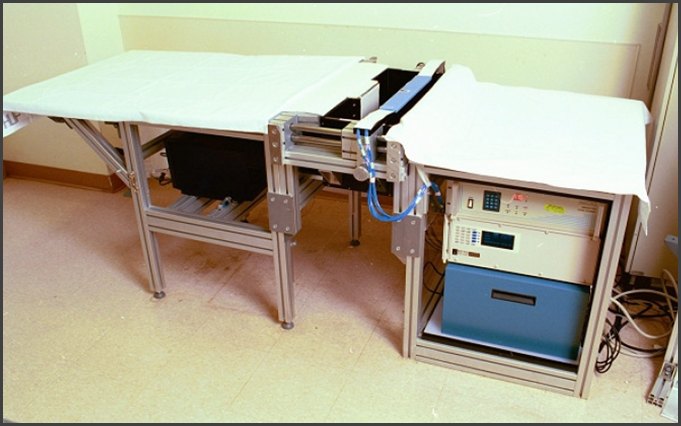
\includegraphics[width=12cm]{./figures/4_Gen3/gen2pic.png}
\caption[Photograph of the previous generation Gen2 breast scanner]{Photograph of the previous generation Gen2 breast scanner located at the Hospital of the University of Pennsylvania (HUP).}
\label{fig:gen2pic}
\end{figure}
\begin{figure}[ht]
\centering
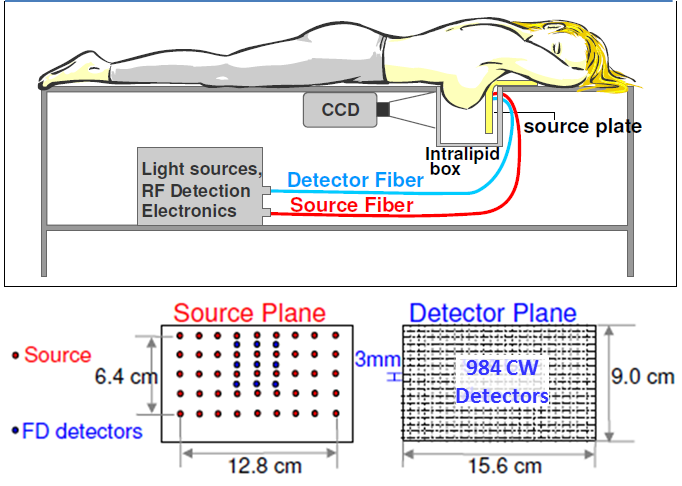
\includegraphics[width=12cm]{./figures/4_Gen3/gen2schem.png}
\caption[Schematic of the Gen2 breast scanner]{Schematic of the Gen2 breast scanner. CW transmission and frequency-domain (FD) remission measurements are taken simultaneously. The patient lies prone, and her breast is compressed axially with the sources and FD detectors on top of the breast and the CCD detection window against the bottom of the breast. The source plate consist of 45 source positions and 9 FD detectors with 16mm spacing between the sources. For the CW transmission measurements, a subset of 984 detectors (pixels) with $3\,{\rm mm}$ spacing is selected from the CCD for reconstruction. This Figure is adapted from a similar schematic by R. Choe \cite{Choe2005}}
\label{fig:gen2schem}
\end{figure}

The DOT measurement is made with the patient lying prone on a flat bed with her breast inserted inside a recessed box. This box has a grid of source fibers on one side (source plate) and a window on the other side (detector plate). The source plate is translated axially to softly compress the breast between the source and detector plates. The box is filled with a matching fluid whose optical properties are similar to those of the average human breast. The matching fluid consists of water, india ink (for absorption) and Intralipid (for scattering). 

The Gen2 source plate has 45 fiber positions arranged in a 9x5 square grid with a spacing of 16 mm between nearest neighbors (Figure~\ref{fig:gen2schem}). The light is launched in series into the medium using cascading optical switches (DiCon Fiber Optics). At each source position, up to six different light source wavelengths were switched in from the fiber-coupled diode lasers (e.g., at wavelengths of 650, 690, 750, 785, 830, 905 nm). On the detection side, a CCD camera (Roper Scientific, Trenton, NJ, VersArray:1300F) collected the exiting light in the transmission geometry. A full CCD image is thus obtained for each source (and each laser/wavelength combination) with an exposure time of ~500 ms. From each image, a grid of data is selected from the CCD after a $2\times 2$ hardware binning of its pixels. For the frequency-domain remission measurements, typically four lasers ($690, 750, 786,$ and $830~\rm{nm}$) are modulated at $70\,{\rm MHz}$; measurements are made in remission with 3 mm diameter detector fibers arranged on the source plate in a $3\times3$ grid with $16\,{\rm mm}$ spacing. The light from these remission fibers are collected by an avalanche photodiode for homodyne frequency-domain analysis.

Of course, much was learned using this device, and these studies informed the design and development of my current DOT breast imager. Perhaps most significantly, it was particularly difficult to eliminate cross-talk between tissue absorption and scattering when employing only CW measurements (see Chapter 2). This difficulty is well known in the community; it arises because both tissue parameters (i.e., scattering and absorption) attenuate detected diffuse light when the intervening medium is turbid (e.g., like breast tissue). By using multi-spectral measurements in transmission and sparse frequency-domain measurements in remission, we were able to ameliorate this problem to some degree. However, it was apparent that the apparatus would benefit from a full frequency-domain approach, an approach that I incorporate in my Gen3 instrument with \textit{heterodyne} detection techniques. 

Another problem concerned breast compression. The Gen2 instrument carried out breast compression in the axial geometry. For comparison to other medical imaging techniques such as MRI, however, the sagittal compression geometry is better and more common than the axial. The Gen3 device employs sagittal compression. Furthermore, a rotation stage in the Gen3 instrument enables DOT measurements in both sagittal and axial compression geometries. 

Still another problem concerned instrumental drifts during the patient data-taking period. We did not measure these drifts \textit{in situ}  with the Gen2 instrument. As will be described later in the chapter, I implement two types of reference signals for real-time normalization in the new instrument.

In addition, we employed (in Gen2) only very crude means to define the breast boundaries. For example, we used the primary CCD camera image of the breast (before adding Intralipid) to indicate the position of the breast boundary and then we approximated the remainder of the boundary as an ellipsoidal 3D surface. Improvements on this scheme for specification of the breast boundaries should lead directly to improvements in DOT image reconstructions. 

Finally, the patient interface needed improvements to increase patient comfort, breast coverage, and to reduce the extent of the air-Intralipid boundary present in the Gen2 instrument configuration. Taken together, all of the noted limitations and potential improvements (as well as the substantially larger amount of data that was possible to obtain with Gen3) motivated us build a whole new instrument system.

\section{Clinical Breast Imaging Device (Gen3)}
\label{sec:Gen3}
The instrumentation and schematic for the Gen3 clinical breast imager that I built is shown in Figures~\ref{fig:gen3schem}, \ref{fig:gen3pic}, \ref{fig:gen3comppic}, \ref{fig:gen3hydraulics}, \ref{fig:gen3rackpic}, \ref{fig:gen3headrest}, and \ref{fig:gen3tank}. Here, the patient lies prone and perpendicular to the modified biopsy bed (Figure~\ref{fig:gen3pic}) while one breast is centered and sagittally compressed between the source plate and window in the breast tank (Figure~\ref{fig:gen3headrest}). Typical thickness of compression varies between $56\,{\rm mm}$ and $70\,{\rm mm}$. As before, the tank is filled with a solution of Intralipid and india ink mixture to match with the tissue optical properties of the patient in the near-infrared (NIR) wavelength range.
%
\begin{figure}[h]
\centering
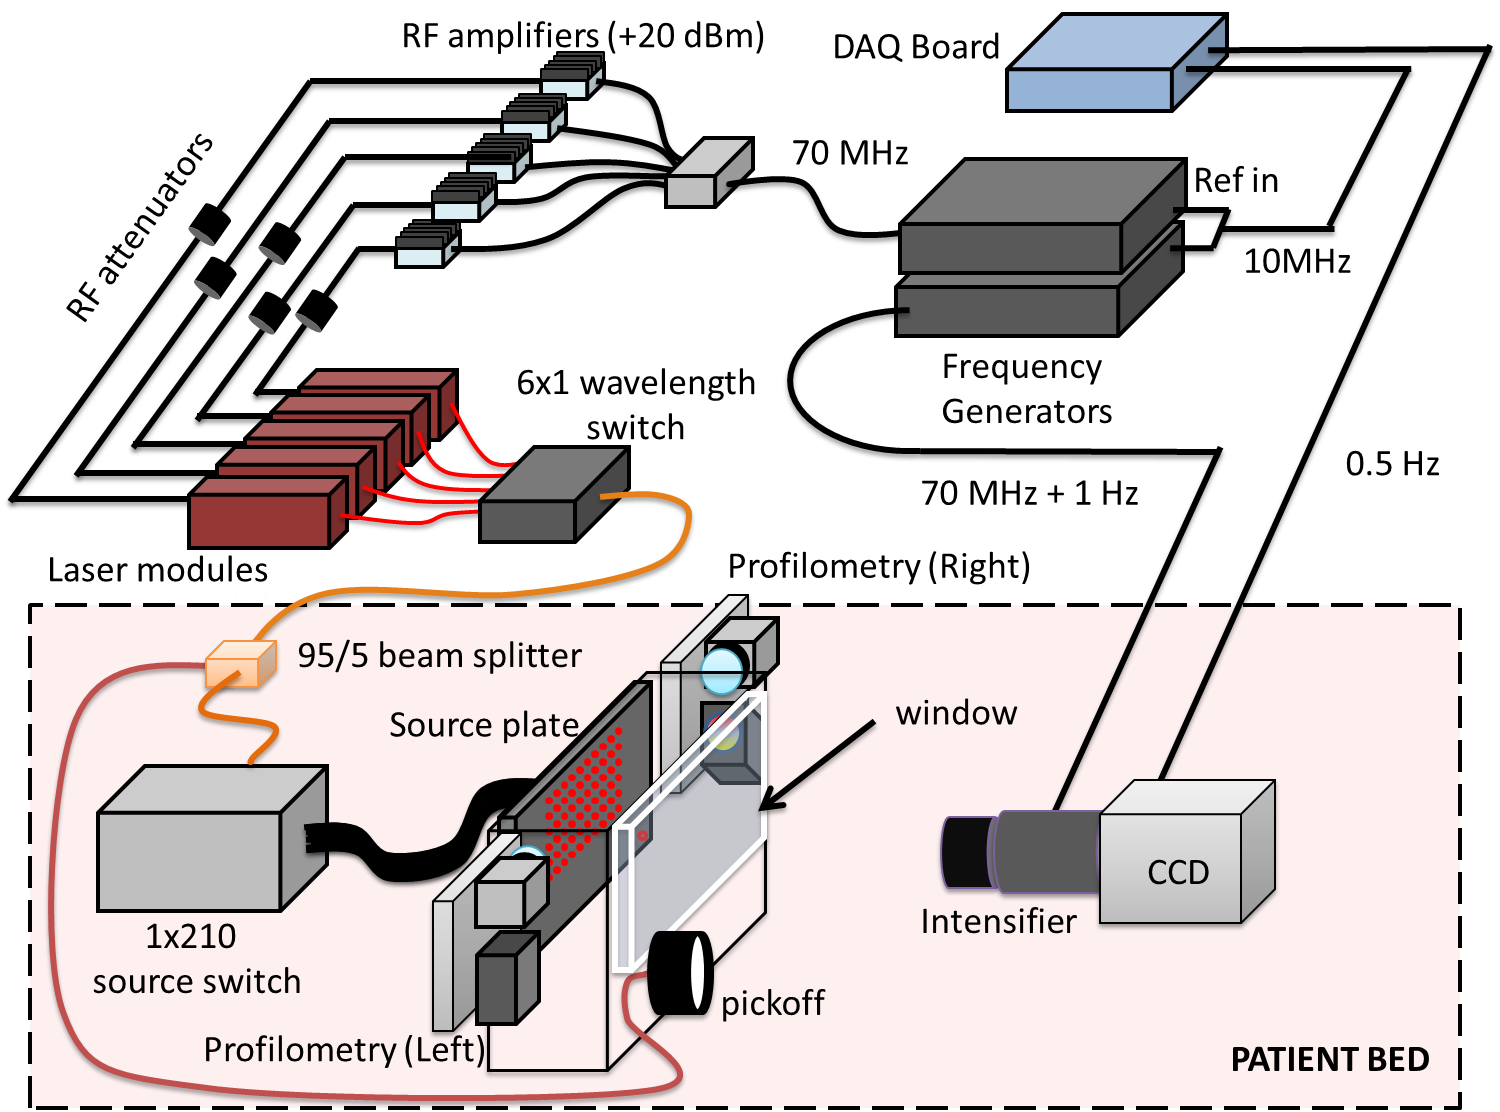
\includegraphics[width=14cm]{./figures/4_Gen3/gen3schem.png}
\caption[Schematic of the Gen3 DOT breast imager]{Schematic of the DOT breast imager. The source-lasers and detection-system are RF modulated at slightly different frequencies. Five RF modulated laser modules are switched through each source position (in series) to yield multi-spectral data. A $210$ channel galvo switch directs the laser light to 209 source positions and a calibration source on the input plate. The patient breast is inserted in the tank between the source plate and window. Profilometry devices on either side of the tank image the “sides” of the breast. Laser light exiting the tank window is measured by a RF gain-modulated intensifier and CCD.}
\label{fig:gen3schem}
\end{figure}
%
\begin{figure}[h]
\centering
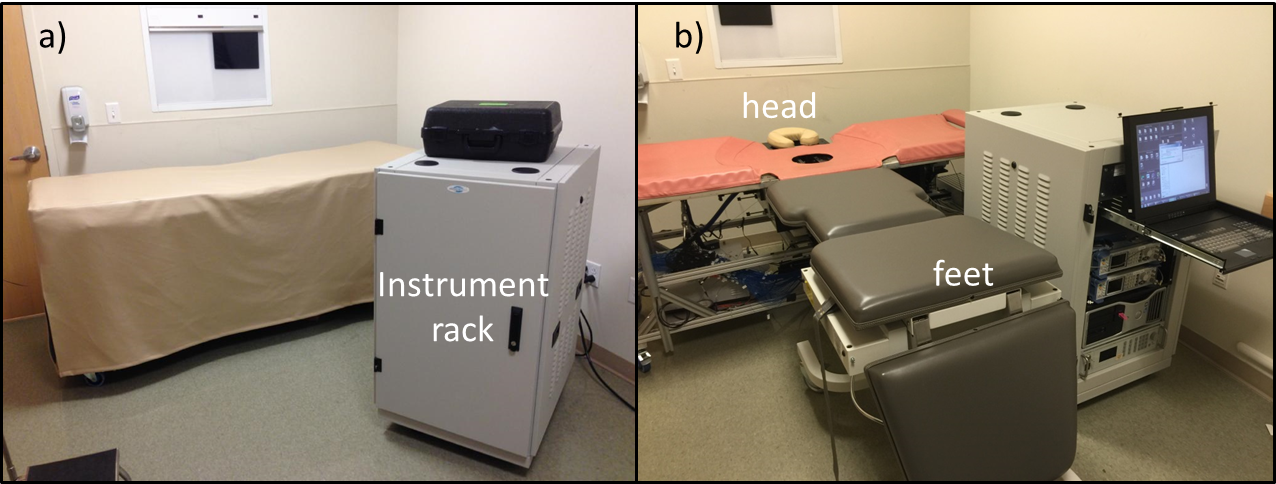
\includegraphics[width=14cm]{./figures/4_Gen3/gen3pic.png}
\caption[The breast imaging instrumentation in the mammography wing of Perelman Center for Advanced Medicine at the Hospital of the University of Pennsylvania (HUP)]{The breast imaging instrumentation in the mammography wing of Perelman Center for Advanced Medicine at the Hospital of the University of Pennsylvania (HUP). a) Gen3 instrument when not in use. b) Gen3 instrument set up for patient measurement. The patient would lie in the prone position with her head on the head rest and body along the grey exam table. More details about each sub-part of the instrument will be given throughout this chapter.}
\label{fig:gen3pic}
\end{figure}

The breast imager has several key components. Briefly, the laser system encompasses optics and electronics for generating frequency-modulated source light at various NIR wavelengths. This light is sent through a custom switch to one of $209$ source positions on the inside a breast tank wherein the breast is inserted. The breast tank has two sets of profilometry cameras and projectors for determination of the breast boundary which, in turn, facilitates 3D segmentation for image reconstruction. Finally, gain-modulated detection is applied to the transmitted light using an image intensifer mounted on the CCD-camera apparatus.

First and foremost, my DOT breast imaging device improved on the Gen2 instrument through the incorporation of multispectral frequency-domain (FD) laser source illumination and CCD-based heterodyne detection; the latter was enabled by gain-modulation of an image intensifier placed between the sample output and the CCD-detector. These new capabilities improve separation of tissue absorption from tissue scattering and thus improve the quantification capability of the 3D DOT reconstruction. Furthermore, by using an improved CCD camera for detection, we were able to collect a very large number ($10^6$) of source-detector pairs in parallel, again facilitating improved resolution and image fidelity. In fact, my instrument collects the largest number of source-detector pairs compared to any DOT instrument in the world today, e.g., by factors of 100x or more. I will describe how these components work in later sub-sections of this chapter.
\begin{figure}[p]
\centering
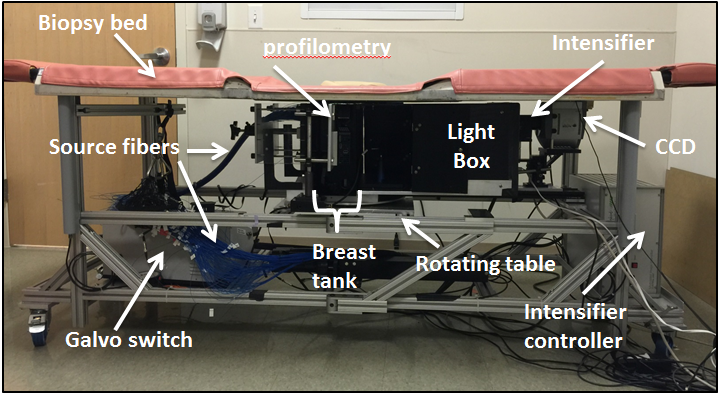
\includegraphics[width=14.5cm]{./figures/4_Gen3/gen3comppic.png}
\caption[Photograph of the of the Gen3 bed with components shown]{Photograph of the of the Gen3 bed with components shown. The bed frame was constructed using $80/20$ Industrial erector set for easy modification.}
\label{fig:gen3comppic}
\vspace{10mm}
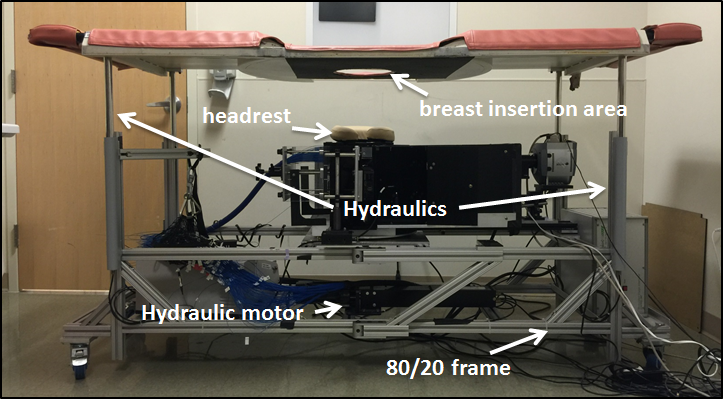
\includegraphics[width=14.5cm]{./figures/4_Gen3/gen3hydraulics.png}
\caption{Hydraulic system installed on the Gen3 bed for maintenance and setup. It is motorized to be able to lift the heavy stainless steel bed.}
\label{fig:gen3hydraulics}
\end{figure}

The temperature in the hospital is not be well controlled (i.e., compared to typical physics labs), and the shift from CW to FD electronics makes the instrument susceptible to long term drifts and signal jitter. These issues are especially important when working with RF electronics and long optical fibers ($>5\,{\rm m}$). To address these issues, we have engineered both front-end solutions such as RF shielding and temperature control to improve laser signal stability, and we have also introduced \textit{active concurrent reference measurements} for real time signal correction and normalization. These improvements are novel and are further discussed in Section~\ref{sec:gen3pp}.
\begin{figure}[h]
\centering
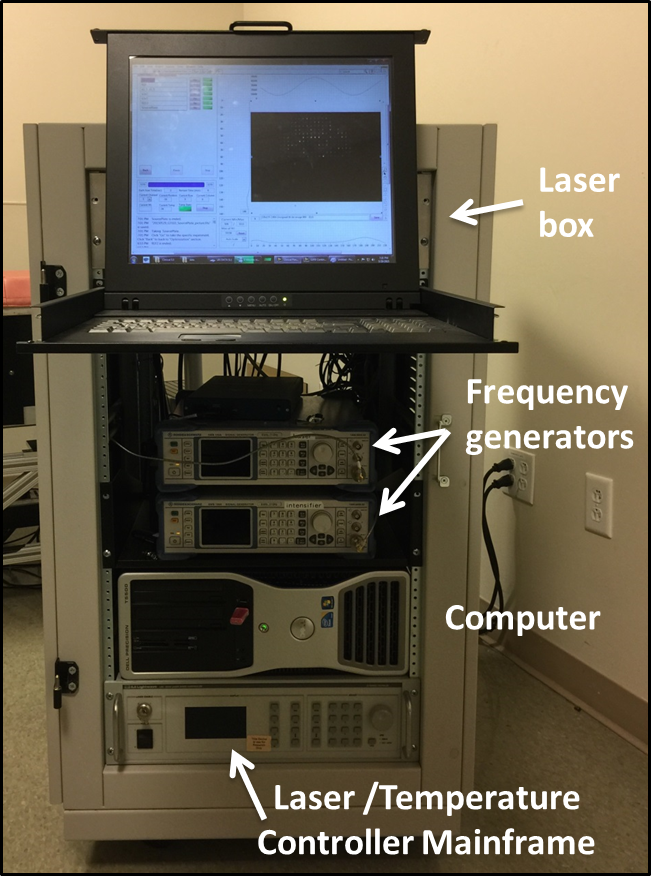
\includegraphics[width=7cm]{./figures/4_Gen3/gen3rackpic.png}
\caption[Photograph of the instrument's primary electronics rack and related components]{Photograph of the instrument's primary electronics rack and related components. This rack contains most of the electronics, as well as the computer that run the Gen3 device. The rack is set next to the patient bed.}
\label{fig:gen3rackpic}
\end{figure}

As noted above, every 3D reconstruction can benefit from knowledge of the breast boundary. In principle, one could use the slab boundary conditions and reconstruct the breast boundary directly; in practice, however, if one knows the location of the breast boundary, then one can segment the reconstruction and substantially reduce the number of unknowns in the inverse problem. To this end, a pair of profilometry imaging systems were designed and were built into the new instrument to provide 3D surface information about the breast shape (discussed in Section \ref{sec:profilometry}). This ancillary instrumentation required overcoming several engineering challenges, e.g., capturing images in the same compression condition as the DOT data, building opto-electronics to work in  small spaces (e.g., imaging within $<6cm$ spacings), compensating and calculating surface information over areas wherein direct imaging could not be carried out, and developing fast acquisition speeds in hardware and software.

Finally, significant effort was made to build a clinical grade device with a patient interface that maximized comfort and minimized movement during measurement. To this end, we designed the bed around a modified breast needle biopsy bed. Since the biopsy bed is designed for maximum breast insertion underneath the bed, we also benefit from resulting greater access to tumors that lie closer to the chest wall. In addition, significant effort was devoted to the design of software for the imager to enable simple and streamlined operation by our clinical collaborators who have minimal technical training. These improvements are further detailed in Section~\ref{sec:clinicalui}.

\subsection{Breast Tank and Patient Bed}
The breast imaging system is built around a modified biopsy patient bed (Figure \ref{fig:gen3comppic}). The bed permits more of the breast to be inserted into the tank for greater breast coverage, i.e., compared to Gen2. A minor but ultimately important improvement was a translating head-rest that was added to improve neck positioning and comfort (Figure~\ref{fig:gen3headrest}). The improved patient comfort led to reduced patient motion. In addition, an ultrasound bed permitted the patient to lie perpendicular to the biopsy bed which further improved patient comfort, ease of measurement, and measurement mechanical stability.

The breast tank is located beneath the hole in the biopsy patient bed. The tank consists of a source plate made from black Delrin that is rail-mounted to maintain parallel alignment between the source plate and window during compression. On the opposite side is an acrylic window with an anti-reflective coating in the NIR (Figure~\ref{fig:gen3tank}). The space between the window and the detection setup is covered by a light box with an inner lining made of black felt that prevents stray light from reaching the image intensifier and CCD. The tank is mounted above a ball-bearing surface which permits the breast tank, light box, and detection system to rotate 90 degrees for either sagittal or axial compression of the breast. The tank is designed to be fitted with a plastic bag (polyethylene, 3mil) so that the tank can be filled with Intralipid solution. Using an optically matching solution compensates for the uneven thickness of the compressed breast, reducing the dynamic range of the transmitted light signal and boundary effects.
%
\begin{figure}[p]
\centering
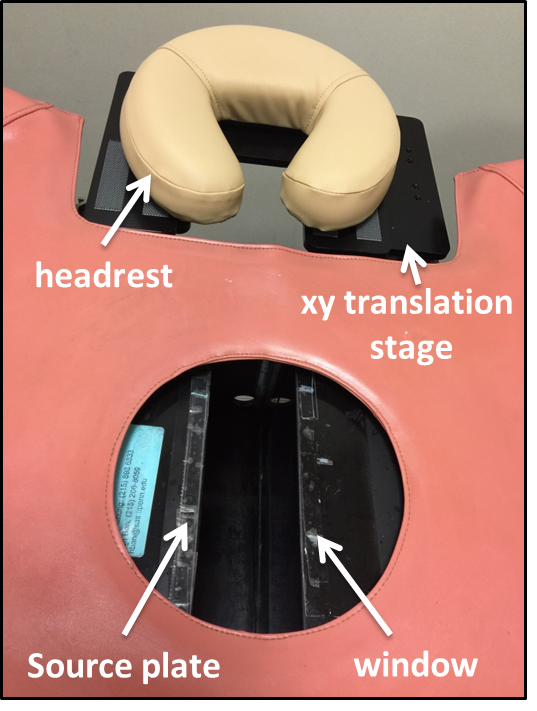
\includegraphics[width=7cm]{./figures/4_Gen3/gen3headrest.png}
\caption[Photograph of the bed headrest and breast insertion area.]{Photograph of the bed headrest and breast insertion area. The headrest sits on a translation stage that adjusts for left/right breast positions and height. The breast is compressed between the source plate and the window.}
\label{fig:gen3headrest}
\vspace{10mm}
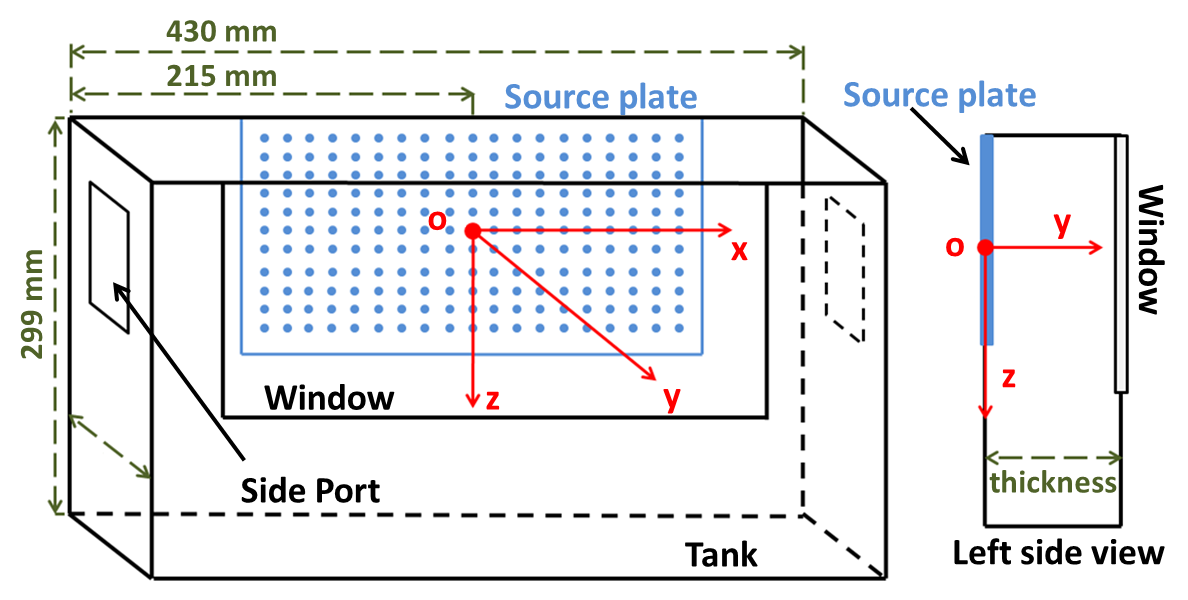
\includegraphics[width=14.5cm]{./figures/4_Gen3/gen3tank.png}
\caption{Schematic of the gen3tank. The coordinates shown are those used in reconstruction and breast profilometry describe in Section~\ref{sec:profilometry}}
\label{fig:gen3tank}
\end{figure}

The frame underneath the bed was custom built with 80/20 aluminum T-slot frames that enable further customization and easy modification in the future. The frame rolls on four castor lock wheels for easy movement and rigidity during measurements. Since the stainless steel bed is of considerable weight, hydraulic lifts (47105T23, McMaster-Carr) in Figure~\ref{fig:gen3hydraulics} were added to aid with maintenance and experiment setup/modification during non-clinical use.

\subsection{Laser System}
Source plate illumination is provided by a set of diode lasers operating at wavelengths of $660$, $690$, $785$, $808$, and $830\,{\rm nm}$, respectively. Table \ref{tab:lasertable} provides detailed characteristics of each laser module (Figure~\ref{fig:laserpic}). The laser output on average is about $80\,\rm{mW}$ from the module fiber tip. The light delivered to the breast ranges in power from $10$ to $15\,\rm{mW}$. The diode lasers are mounted on a custom copper block coupled to a thermistor and a thermoelectric cooler (TEC) for temperature cooling and control at $13^{\circ}{\rm C}$ with stability within $0.1^{\circ}{\rm C}$. Each diode laser is driven and temperature controlled by a dedicated ILX module (LDC 391672, ILX). Note, by comparison, the Gen2 instrument used controllers based around a simple driver (Thorlabs, IP500) and lacked temperature control for its lasers. The CW stability of each laser is quite good as a result of these front-end improvements, i.e., the intensity varies by less than $0.5\%$ over three hour periods. 
%
\begin{figure}[p]
\centering
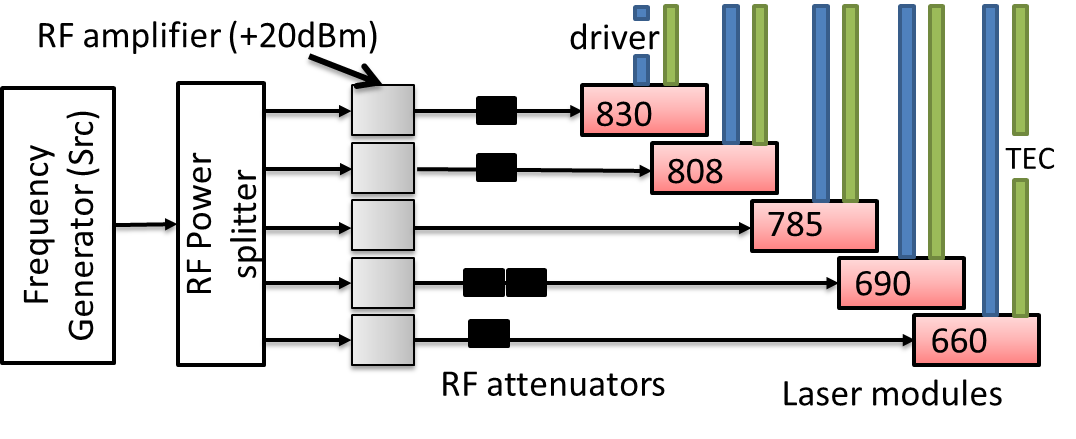
\includegraphics[width=12cm]{./figures/4_Gen3/RFlaser.png}
\caption[Schematic showing laser modules being RF driven]{Schematic showing laser modules being RF driven. Signal from the frequency generator is divided with an RF power splitter. Each branch is amplified then attenuated to appropriate levels optimized for each laser. Each laser module has a driver and TEC control with feedback. The driver provides CW current which is combined with the RF signal inside the module.}
\label{fig:RFlaser}
\vspace{10mm}
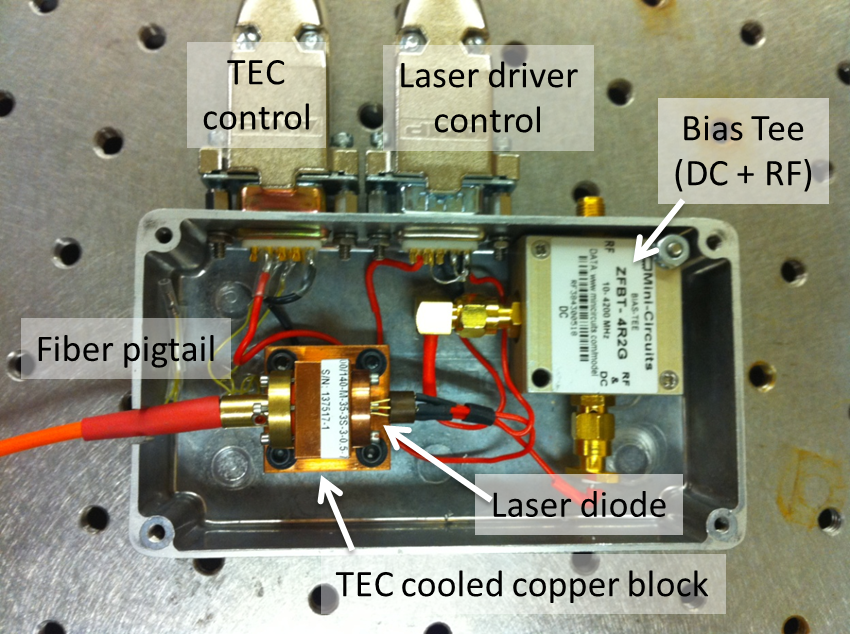
\includegraphics[width=10cm]{./figures/4_Gen3/laserpic.png}
\caption[Photograph and schematic of laser module]{a) Photograph of the laser module. b) Schematic of the laser module. The laser module has three inputs: 1) the RF modulation and 2) the DC current drive, which are combined by the bias-tee; 3) the TEC voltage, which drives the cooling element. The module has two outputs: 1) the photodiode (if available) and the 2) thermistor. These outputs provide feedback for the driver current and temperature control, respectively. The “cold side” of the TEC element cools the copper block to the desired temperature, and heat is released into the module casing.}
\label{fig:laserpic}
\end{figure}

Figure \ref{fig:RFlaser} shows the schematic of the lasers being amplitude modulated at $70\,{\rm MHz}$ using a an RF signal from a frequency generator (Rhode and Schwartz, SMB100). More specifically, the $70\,{\rm MHz}$ RF signal from the frequency generator is combined with the DC current from the ILX driver for each laser with a bias-tee (Mini-circuits, ZFBT-4R2G). The DC and RF voltage input for each laser was optimized using RF amplifiers (Mini-circuits, ZHL-2010+) and RF attenuators (Mini-circuits, VAT series). The laser driver current is optimized for the best modulation depth ($80\%$) and a sinusoidal waveform. The frequency-modulated light from each laser is then fiber coupled to a 6x1 100 $\mu m$ core optical switch (Optojenna) which controls wavelength switching in series. A photograph of the laser box is shown in Figure~\ref{fig:laserbox}.
\begin{figure}[h]
\centering
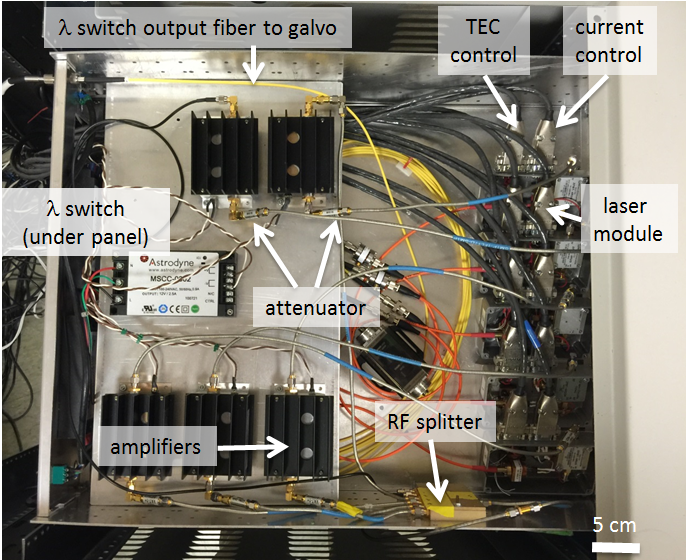
\includegraphics[width=11cm]{./figures/4_Gen3/laserbox.png}
\caption[Photograph of the laser box]{Photograph of the laser box. The RF signal (from frequency generator outside of box) is split into five branches, and each is sent through 20dBm amplifiers and then attenuated to the appropriate voltage for each laser module.}
\label{fig:laserbox}
\end{figure}
\begin{table}[h]
\centering
\begin{tabular}{|c|c|c|c|c|c|c|}
\hline
$\lambda$ & Diode laser & Pin type & spec. current & current &AC input & power\\ 
(nm) & part no. & (Thorlabs) & typ./max (mA) & ILX (mA) & (dBm) & (mW) \\ \hline
660 & HL6545MG & H & 170 / 210 & 110 & 23 & 45 \\
690 & V2561-2 & C & 768 / 800 & 425 & 20 & 96 \\
785 & L785P090 & C & 120 / 160 & 93 & 22 & 67 \\
808 & L808P200 & A & 230 / 300 & 180 & 20 & 80 \\
830 & L830P150 & C & 200 / 250 & 123 & 19 & 78 \\ \hline 
\end{tabular}
\caption[Laser inventory and specifications for the Gen3 device]{Laser inventory and specifications for the Gen3 device. The ILX driver provides the DC current, and the AC modulation is derived from the RF frequency generator. The laser output power is measured at the end of the pigtail fiber from the laser. Throughput loss is $\sim 80\%$ from the laser module to the source plate.}
\label{tab:lasertable}
\end{table}
\subsection{Source Position Switch and Source Plate}
\label{sec:sources}
The output fiber from the wavelength switch is connected in series to a $95/5$ fiber beam splitter with the $5\%$ going to the pickoff for signal normalization (which will be discussed in Section \ref{sec:gen3pp}), and $95\%$ going to a custom 1x210 channel optical galvo-switch (Figure~\ref{fig:gen3switchschem}). We upgraded Gen3 to employ a galvo-switch for several reasons. By comparison, the Gen2 system switched through 210 channels with a conventional switch cascade, based on mechanical or prism mechanisms, and it was costly, slow, and had high throughput losses. The Gen2 system switching speed between sources ranged from $0.3$ to $0.5\,{\rm s}$ and had an average throughput of $50\%$. More importantly, the Gen2 switches had throughput heterogeneity which ranged from $10\%$ to $80\%$ and which resulted in SNR variation between sources.

The Gen3 galvo-switch, by contrast, has more uniform throughput, i.e., with differences in intensity between sources no greater than $10\%$. In the galvo switch, input light from a $100\,\mu{\rm m}$ core fiber is collimated and sent towards galvo-controlled mirrors which then redirect light into a telecentric lens. This lens focuses the light onto a fiber bundle face with 210 fibers ($600\,\mu{\rm m}$ core) as shown in Figure~\ref{fig:gen3switchpic}. Each fiber from the bundle is connected to a custom source fiber with $600\,\mu{\rm m}$ core. The source fibers were hand-polished (to achieve $98\%$ throughput) and fitted with FC/PC connector on the end towards the fiber bundle, and a custom ferrule on the end connecting to the delrin source plate.

The 209 source fibers are arranged on an 11x19 square grid on a black delrin plate with 8 mm spacing. The source plate is moved against the detection window and a picture is taken to determine source positions for reconstruction as shown in Figure~\ref{fig:srcplatepic}. One of the remaining fibers is used as a calibration source and is thus placed far from the source grid. The purpose and implementation of this calibration source will be discussed in Section~\ref{sec:gen3pp}.
\begin{figure}[p]
\centering
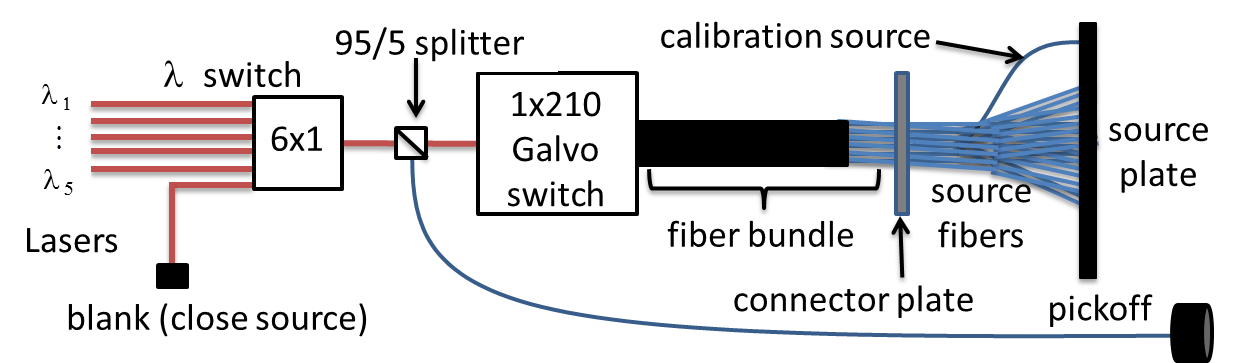
\includegraphics[width=14cm]{./figures/4_Gen3/gen3switchschem.png}
\caption[Schematic of switches and fibers in the Gen3 system]{Schematic of switches and fibers in the Gen3 system. The output light from the laser modules are fiber-coupled to a $6\times 1$ wavelength switch. Output of the wavelength switch is then directed through a beam splitter with $5\%$ going to a pickoff source which is used as an instrument source reference. The remainder is input to a $1\times 210$ galvo switch which redirects the light into one of $210$ channels of a fiber bundle. The fiber bundle is connected via custom source fibers to the source plate. $209$ of the fibers are arranged in a $11\times 19$ square grid with $8\,{\rm mm}$ separation, and one of the channels is used as a (second) calibration source placed far from the breast measurement area.}
\label{fig:gen3switchschem}
\vspace{10mm}
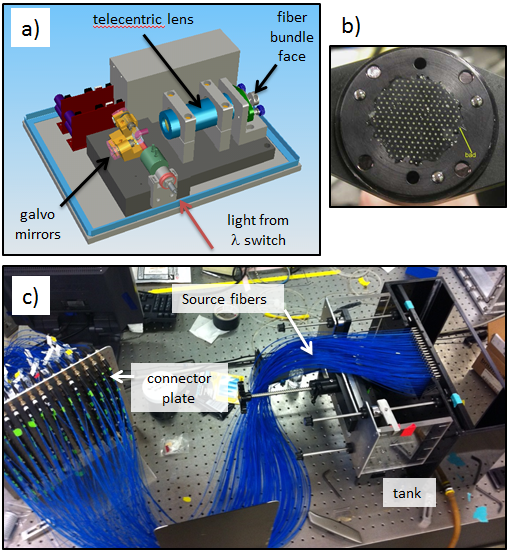
\includegraphics[width=10cm]{./figures/4_Gen3/gen3switchpic.png}
\caption{Photograph of the (a) galvo switch, (b) the input face of the fiber bundle, and (c) the custom source fibers and source plate}
\label{fig:gen3switchpic}
\end{figure}
\begin{figure}[h]
\begin{center}
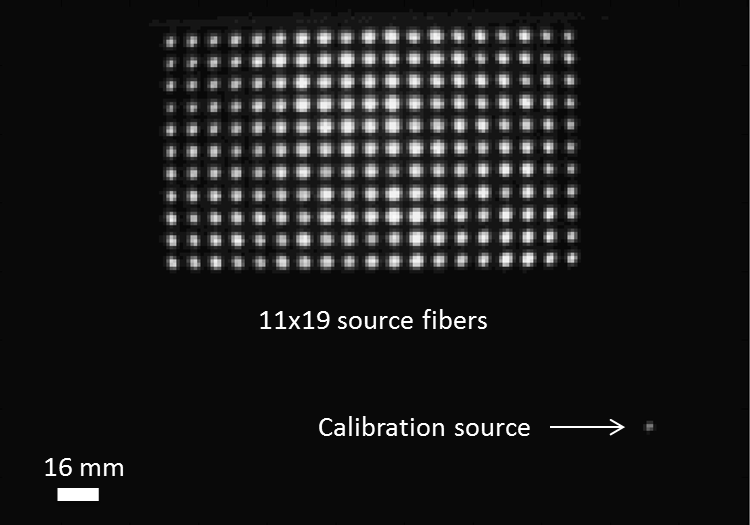
\includegraphics[width=10.5cm]{./figures/4_Gen3/srcplatepic2.png}
\caption[Source plate photograph taken by the Breast Imager CCD after it has been moved to the detection window]{Source plate photograph taken by the Breast Imager CCD after it has been moved to the detection window. The fibers are lit by illuminating the back end of the fiber bundle. In practice, this image is used to provide fairly precise estimates of the source positions for the tomographic reconstructions. The spacing between sources are $8 {\rm mm}$ between nearest neighbors.}
\label{fig:srcplatepic}
\end{center}
\end{figure}
\begin{figure}[h]
\begin{center}
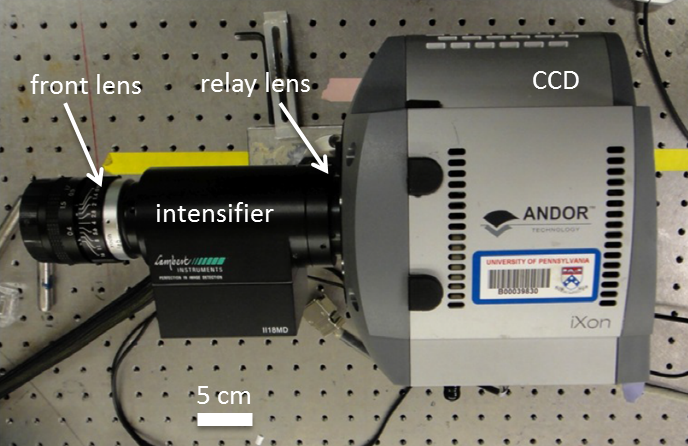
\includegraphics[width=10.5cm]{./figures/4_Gen3/camerapic.png}
\caption{A photograph of our CCD with a Lambert instruments image intensifier mounted in the front.)}
\label{fig:camerapic}
\end{center}
\end{figure}
%
\subsection{Image Intensifier mounted CCD}
\label{sec:CCD}
The detection system consists of a back-illuminated EMCCD (Andor iXon DV887, Ireland) with quantum efficiency optimized in the $500-700\,{\rm nm}$ range as shown in Figure~\ref{fig:camerapic}. One of the most attractive features of this CCD is its ``frame transfer" function which permits \textit{shutterless} continuous measurement; this feature is beneficial for our heterodyne measurement scheme which is described in Section \ref{sec:heterodyne}. CCDs with frame transfer options feature a second CCD chip that acts as a buffer while the first chip continues to be exposed. The speed at which it shifts the data to this secondary chip is roughly $3\,{\rm \mu s}$ per row of pixels. This allows for a series of exposures to be taken continuously without a need for a mechanical shutter. The $512 \times 512$ pixel CCD is cropped to a field-of-view corresponding to the breast tank window; with a $2 \times 2$ hardware binning this set up produces an image $155 \times 200$ pixels with a dpixel of $1.2268\, {\rm mm/pixel}$ with a 16-bit depth. The CCD is mounted together with a relay lens and with a gain-modulated image intensifier (Lambert Instruments, II8MD GENIII, Netherlands) that has a P43 Phosphor screen with a peak emission at $545\, {\rm nm}$. The lens element in front of the image intensifier is a Xenon $25\,{\rm mm}$ $f/0.95$ C-Mount Lens for 1-Inch CCD (Schneider Optics, Germany).
\begin{figure}[h]
\begin{center}
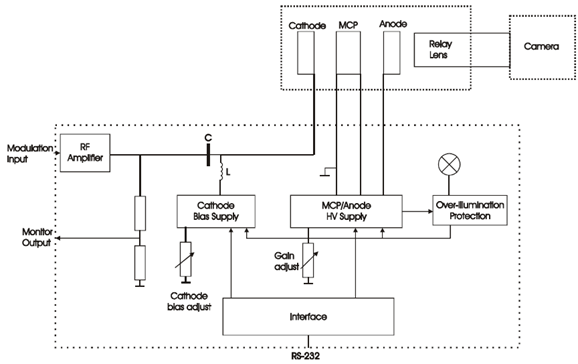
\includegraphics[width=14cm]{./figures/4_Gen3/iischem.png}
\caption[Schematic of the image intensifier electronics]{Schematic of the image intensifier electronics. The cathode converts light into electrons which are amplified by the MCP. The image intensifier gain is RF modulated at the cathode. (\textit{Figure from Lambert Instrument manual for II8MD})}
\label{fig:iischem}
\end{center}
\end{figure}

Briefly, the image intensifier works by converting light into electrons which are then amplified electronically before being converted back to light again (at the phosphor screen). Specifically, incident light on the cathode (coated with a photosensitive compound) of the image intensifier is converted to electrons via the photoelectric effect. When the voltage applied to the cathode is negative, a potential difference between the cathode and anode is created and causes electrons to move (accelerate) towards the anode. When a positive voltage is applied to the cathode, the image intensifier is effectively "off"; the electrons do not escape to the anode. When the intensifier is on, the electron travels through the multichannel plate (MCP) and the number of electrons is amplified/increased. These electrons are converted back into light when they strike the phosphor screen at the back of the intensifier. This “amplified” light signal is then focused onto the CCD by the relay lens. The electronic schematic for this process is shown in Figure~\ref{fig:iischem}. The gain on the image intensifier is modulated at the cathode with a frequency of $70\,{\rm MHz} + 1 {\rm Hz}$, thereby permitting \textit{heterodyne} detection as described in the next section.
%
\subsection{Frequency-Domain Heterodyne detection}
\label{sec:heterodyne}
The primary goal of the frequency-domain DOT system is to measure the AC amplitude and phase components of the signal for each source detector pair. Generally, two approaches are used to demodulate a high frequency RF signals: homodyne and heterodyne. Several homodyne systems have been developed for diffuse optical imaging \cite{Troy1996,Sevick-Muraca1997,Godavarty2003}, including in our lab, but here we describe the heterodyne approach. The heterodyne approach usually has better signal-to-noise than homodyne schemes, as the signal can be filtered and is received at the cross-correlation frequency ($f_{cc}$); by working away from zero-frequency, the heterodyne measurement exposure to so-called pink ($1/f$) noise (and other noise) is less \cite{Venugopal2012}. Heterodyne detection also better enable concurrent amplitude and phase corrections via the pickoff normalization/calibration signals thereby facilitating corrections to long-term drifts (see Section~\ref{sec:gen3pp}.

Our system uses an optical heterodyne detection scheme wherein an input source is modulated at frequency, $f_{s}$, is mixed (nonlinearly) with a reference detection signal modulated at a similar frequency $f_d=f_{s}+f_{cc}$ where $f_{cc}=1~{\rm Hz}$. In our instrumentation, the reference signal is used to alter the detector gain. The result is that the detected light signal has a component that oscillates at the beat frequency $f_{cc}$ from which the amplitude and phase data can be extracted. In our system, the modulation frequencies at $f_{s}$ and  $f_{d}$ are provided by a pair of phase-locked frequency generators (Rohde and Schwarz, SMA100A). 

The lasers are amplitude modulated at $f_{s}=70\,{\rm MHz}$. Therefore, the light source power density in the sample entrance is given by
\begin{equation}
S_s(\mbf{r}_s,t) = S_{dc}(\mbf{r}_s) + S_{ac}(\mbf{r}_s)\cos(2\pi f_s t) \ .
\end{equation}
\noindent
Here the angular frequency and the frequency are related according to $f=\omega/2\pi$, and $\mbf{r_s}$ denotes the spatial position of the source. For example, for a point-like source, the source function would be a delta function in space. (Note, unlike Chapter 2, here we are not using complex notation for the source and fluence rate.) When the light passes through the breast tank (i.e., through breast and/or Intralipid solution), then the measured fluence rate, $\Phi$, will be of the form
\begin{equation}
\label{eqn:FDfluence}
\Phi(\mbf{r}_s,\mbf{r}_d,t) = \Phi_{dc}(\mbf{r}_s,\mbf{r}_d) + \Phi_{ac}(\mbf{r}_s,\mbf{r}_d)\cos(2\pi f_s t + \theta(\mbf{r}_s,\mbf{r}_d)) \ .
\end{equation}

Here $\Phi_{dc}$, $\Phi_{ac}$, and $\theta$ represent the DC amplitude, AC amplitude and AC phase shift, respectively. These factors all depend on source and detector positions; of course, in addition, the properties of the medium are impressed onto the light fluence-rate as it traverses the medium from the source position $\mbf{r}_s$ to detector position $\mbf{r}_d$. Thus, these are the functions that contain information about the sample. This information about the sample properties is ultimately derived from the data via DOT inversions (see Chapter 2). The inversions yield optical absorption and scattering coefficients, i.e., tissue optical properties. Herein I will drop $\mbf{r}_s$ and $\mbf{r}_d$ and assume that the equations refer to diffuse light measured for a specific source-detector pair (i.e., a single light source and a single pixel detector); these omissions simplify notation in the equations below.

The detection gain response of the image intensifier is shown in Figure~\ref{fig:iigain}. The gain is controlled by the voltage level applied to the cathode. In our experiments, we apply a reference RF voltage signal to the cathode which has both DC offset and AC voltage modulation. The reference modulation frequency is $f_d$. When the voltages are set properly, the reference signal turns the image intensifier gain on and off and thus produces a time-dependent gain. This time-dependent gain effectively serves as a diffuse light signal sampler which, in turn, enables us to derive $\Phi_{ac}$, and $\theta$.

Specifically, the cathode DC voltage is set by the intensifier controller, and the AC voltage modulation is derived from the second frequency generator (modulated at $70\,{\rm MHz}+1\,{\rm Hz}$). Typically, the cathode DC offset is set to $0.8\,\rm{V}$ and the amplitude of the AC modulation is set to $1.8\,\rm{V}$. (As an aside, this corresponds to a frequency generator output setting of $-13\,\rm{dBm}$.) The gain is "off" until the modulation causes the bias to run up and down the linear part of the gain curve at cathode voltages below $-1\rm{V}$, as shown in Figure~\ref{fig:iigain}. The overall effect of this reference modulation signal is to produce a gated gain curve with frequency $f_d$; the gain modulation is essentially a series of pulses with narrow time-width and a repetition period set by the reciprocal of $f_d$.  This method is a commonly used technique for gated detection and sampling.

In our analysis, we will approximate the time-dependent gain function by a series of Dirac delta functions; the delta functions peak at $t=nT_d$, where $T_d = 1/f_{d}$ and $n$ is an integer. In our instrument, of course, each pulse in the comb will have a finite temporal width, but this width will only change our results by a proportionality constant.  

\begin{figure}[h]
\begin{center}
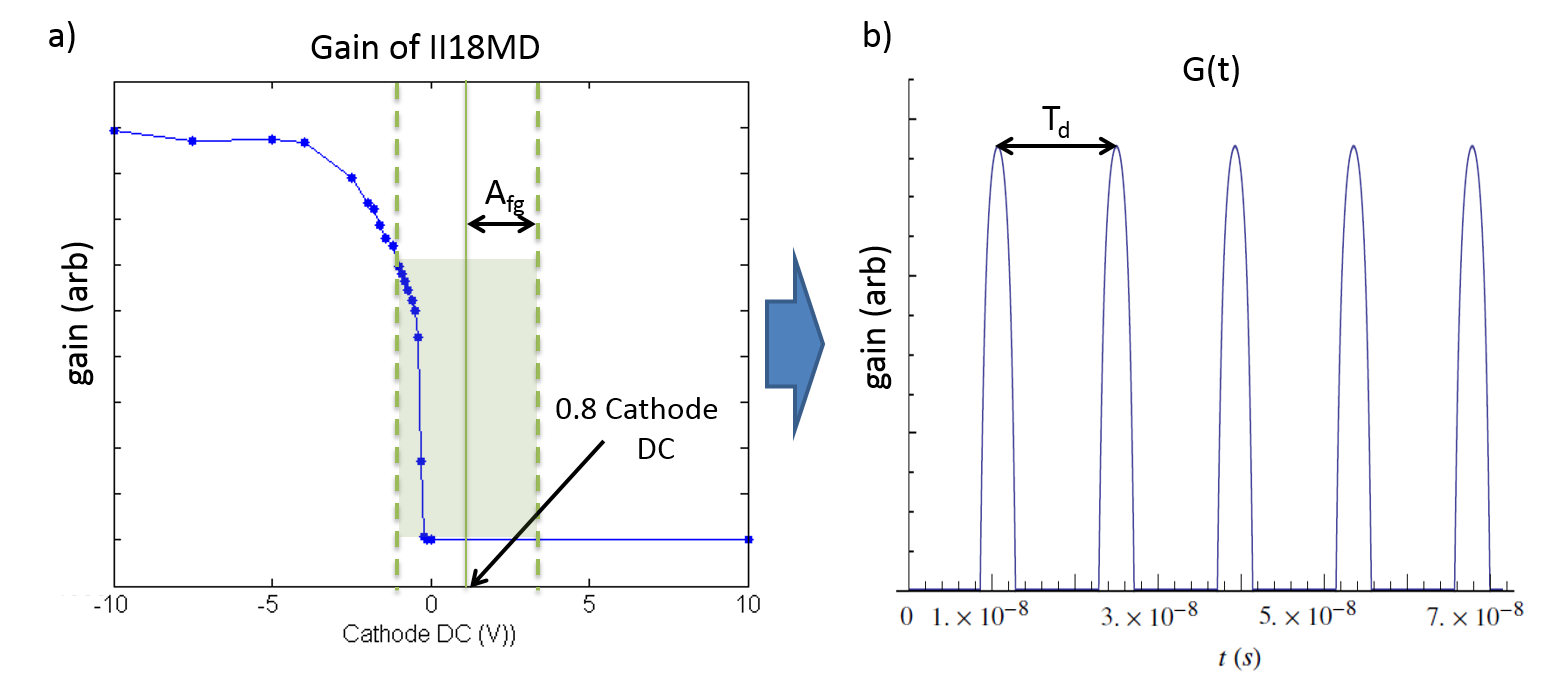
\includegraphics[width=14.5cm]{./figures/4_Gen3/iigain.png}
\caption[Measured gain response curve for the image intensifier for various cathode voltage values]{a) Measured gain response curve for the image intensifier for various cathode voltage values. Green solid line shows where the cathode DC value is set to $0.8\,\rm{V}$. Shaded region between dotted lines show the input AC voltage modulation range from the frequency generator with an amplitude of $1.8\,\rm{V}$. b) Schematic of intensifier gain as a function of time (due to the reference modulation). These curves will be approximated as a comb of delta functions for the analysis.}
\label{fig:iigain}
\end{center}
\end{figure}

We thus model our detection system gain as a Dirac comb of pulses modulated at $70\,\rm{MHz} + 1\,\rm{Hz}$. The equation for the gain, in this case, is:
\begin{equation}
\label{eqn:diraccomb}
G(t)\equiv\sum_{n=-\infty}^{\infty} G_0\,\delta(t - nT_d) \ .
\end{equation}
\noindent
where $G_0$ is some effective gain constant which will ultimately be normalized out and $T_d=1/f_d$ is the repetition period of our gain modulation. The measured signal, $M$, at the CCD is therefore simply the product of Equation~\ref{eqn:FDfluence} and \ref{eqn:diraccomb}:
\begin{align}
M(t)
&=\Phi(t)G(t) \notag\\
&=\left(\Phi_{dc} + \Phi_{ac} \cos(2 \pi f_s t+\theta)\right)\left( \sum_{n=-\infty}^{\infty}G_0\,\delta(t-n T_d)\right) \ .
\end{align}

To further simplify this equation we will utilize the convolution theorem. To do so we take the Fourier transform of the fluence rate and gain. The Fourier transform for the fluence rate is
\begin{align}
\label{eqn:srcFT}
\hat{\Phi}(f) 
&=\int_{-\infty}^{\infty} \left(\Phi_{dc}+\Phi_{ac} \cos(2 \pi f_s t+\phi)\right) e^{- 2 \pi i f t} dt \notag \\
&=\Phi_{dc} \delta(f) + \frac{\Phi_{ac}}{2} \left( \delta(f-f_s)e^{i\theta}+\delta(f+f_s)e^{-i\theta}\right) \ .
\end{align}
The Fourier transform of a Dirac comb is
\begin{align}
\label{eqn:diracFT}
\hat{G}(f)
&=\frac{1}{T_d}\sum_{n=-\infty}^{\infty} G_0\,\delta\left( f - \frac{n}{T_d}\right) \ .
\end{align}
\noindent
Now the convolution of Equation~\ref{eqn:srcFT} and \ref{eqn:diracFT} is
\begin{align}
\label{eqn:Mconv}
\hat{M}(f)
&=\hat{\Phi}*\hat{G} \notag\\
&=\int_{-\infty}^{\infty} \left[\Phi_{dc} \delta(f') + \frac{\Phi_{ac}}{2} \left( \delta(f'-f_s)e^{i\theta} + \delta(f'+f_s)e^{-i\theta}\right)\right] \hat{G}(f-f')df' \notag \\
&=\Phi_{dc} \hat{G}(f)+ \frac{\Phi_{ac}}{2}\left(\hat{G}(f-f_s)e^{i\theta}+\hat{G}(f+f_s)e^{-i\theta}\right) \ .
\end{align}
Using the definition of the Dirac Comb in Equation~\ref{eqn:diraccomb}, Equation~\ref{eqn:Mconv} becomes
\begin{align}
\hat{M}(f) &=\frac{G_0}{T_{d}} \sum_{n=-\infty}^{\infty} \Big[\Phi_{dc}\delta \left( f - \frac{n}{T_{d}}\right) \notag\\
&+ \frac{\Phi_{ac}}{2} \left(\delta \left( f-f_s -\frac{n}{T_{d}}\right)e^{i\theta} + \delta\left(f+f_s-\frac{n}{T_{d}}\right)e^{-i\theta}\right) \Big] \ .
\end{align}
Next, we compute the lower order terms. Expanding the first term ($n=0$) we get
\pagebreak
\begin{equation}
\hat{M}_0(f)=\frac{G_0}{T_{d}}\Big[\Phi_{dc}\delta(f)+\frac{\Phi_{ac}}{2}\Big( \delta(f-f_s)e^{i\theta}+\delta(f+f_s)e^{-i\theta}\Big)\Big] \ .
\end{equation}
\noindent
For which the inverse Fourier transform is
\begin{equation}
M_0(t)=\mathcal{F}^{-1}\Big[\hat{M_0}(f)\Big] =\frac{G_0}{T_{d}}\Big(\Phi_{dc}+\Phi_{ac}\cos(2\pi f_st+\theta)\Big) \ .
\end{equation}
\noindent
For $n=1$
\begin{align}
M_{1}(f)
&=\frac{G_0}{T_{d}}
\left[\Phi_{dc}\delta\left(f-\frac{1}{T_{d}}\right)+\frac{\Phi_{ac}}{2}\left(\delta\left( f-f_s-\frac{1}{T_{d}}\right)e^{i\theta}+\delta \left(f+f_s-\frac{1}{T_{d}}\right)e^{-i\theta}\right)\right] \notag\\
&=\frac{G_0}{T_{d}}\left[\Phi_{dc} \delta(f-f_s-f_{cc})+\frac{\Phi_{ac}}{2}\left(\delta(f-2f_s-f_{cc})e^{i\theta}+\delta(f-f_{cc})e^{-i\theta}\right)\right] \ .
\end{align}
\noindent 
Here I have made the substitution $f_d=f_s+f_{cc}$ in the last step. The corresponding inverse Fourier transform is
\begin{align}
M_{1}(t)
&= \frac{G_0}{T_{d}} \int_{-\infty}^{\infty} \Big[\Phi_{dc}\delta(f-f_s-f_{cc}) \\
& \qquad + \frac{\Phi_{ac}}{2} \left(\delta(f-2f_s-f_{cc})e^{i\theta}+\delta(f-f_{cc})e^{-i\theta}\right)\Big] e^{2 \pi i f t}df \ .
\end{align}
 Similarly for $n=-1$
\begin{align}
M_{n=-1}(t)
&= \frac{G_0}{T_{d}} \int_{-\infty}^{\infty} \Big[\Phi_{dc}\delta(f+f_s+f_{cc}) \\
& \qquad + \frac{\Phi_{ac}}{2} \left(\delta(f+f_{cc})e^{i\theta}+\delta(f+2f_s+f_{cc})e^{-i\theta}\right)\Big] e^{2 \pi i f t}df \ .
\end{align}
Combining $M_1$ and $M_{-1}$ gives us
\begin{align}
M_{1}(t) + M_{-1}(t)
&= \frac{G_0\Phi_{dc}}{T_{d}} \int_{-\infty}^{\infty} \Big(\delta(f-f_s-f_{cc})+\delta(f+f_s+f_{cc}) \Big)e^{2 \pi i f t}df \notag \\
& \qquad + \frac{G_0\Phi_{ac}}{2T_{d}} \int_{-\infty}^{\infty} \Big(\delta(f-2f_s-f_{cc})e^{i\theta} + \delta(f+2f_s+f_{cc})e^{-i\theta}\Big) e^{2 \pi i f t}df \notag \\
& \qquad + \frac{G_0\Phi_{ac}}{2T_{d}} \int_{-\infty}^{\infty} \Big(\delta(f-f_{cc})e^{i\theta} + \delta(f+f_{cc})e^{-i\theta}\Big) e^{2 \pi i f t}df \notag\\
&=\frac{G_0\Phi_{dc}}{2T_{d}} \cos(2\pi f_s t)+ \frac{G_0\Phi_{ac}}{4T_{d}} \cos(2\pi(2f_s+f_{cc})+\theta) \notag\\ 
& \qquad + \frac{G_0\Phi_{ac}}{4T_{d} }\cos(2\pi(f_{cc})+\theta) \ .
\end{align}
\noindent
One can then write down the full series for $M(t)$ as
\begin{align}
\label{eqn:Mfluence}
M(t)
&= \frac{G_0}{T_{d}}\Big(\Phi_{dc}+\Phi_{ac}\cos(2\pi (f_s+f_{cc})t+\theta)\Big) & (M_0\,{\rm term}) \notag\\
& + \frac{G_0\Phi_{dc}}{2T_{d}} \cos(2\pi f_s t)+ \frac{G_0\Phi_{ac}}{4T_{d}} \cos(2\pi(2f_s+f_{cc})+\theta) \notag\\
& + \underline{\frac{G_0\Phi_{ac}}{4T_{d} }\cos(2\pi(f_{cc})+\theta)} & (M_{\pm 1}\,{\rm term}) \notag\\
& + \frac{G_0}{T_d}\sum_{n=2}^{\infty}\Big[\frac{G_0\Phi_{dc}}{2} \cos(2 \pi n f_st) + \frac{G_0\Phi_{ac}}{4}\Big(\cos(2 \pi(f_s-n f_d)t+\theta) \notag\\
& \qquad + \cos(2 \pi(f_s+n f_d)t+\theta)\Big)\Big] \ . & (n\geq 1\,{\rm terms})
\end{align}
This equation provides the light fluence-rate incident on the CCD for a given pixel. Note that one DC and one $1\,{\rm Hz})$ term arise. All other terms oscillate at a frequency of $\sim 70 {\rm MHz}$ or greater.

In the experiment, the response time of the detection is limited by our CCD exposure time which is only very slightly less than $\sim100\,{\rm ms}$ (note also, the frame transfer function of the CCD is $10 \rm{Hz}$). Any term with a modulation frequency greater than $10\,\rm{Hz}$ (and certainly any term in the MHz range) will average to zero:
\begin{align}
\label{eqn:heterodyneresult}
M(t)
& \propto G_0\Phi_{dc} + \underline{\frac{G_0\Phi_{ac}}{4}\cos(2\pi f_{cc} t+\theta)} + 0\,\big(\rm{higher\,freq.\,terms}\big) \ .
\end{align}

Of course, in practice the measurement is scaled with the camera aperature, gain pulse width, exposure time, pixel size, etc., all of which affect the number of electrons that charge up the CCD pixel (and all of which are canceled out by normalization). Equation~(\ref{eqn:heterodyneresult}) is the equation we use to determine the values of $\Phi_{dc}$, $\Phi_{ac}$ and $\theta$ from the raw data. This conversion is the first step in our data preprocessing.

\subsection{DOT measurement and timing}
The measurement timing is controlled using a National Instruments DAQ board (NI USB-6351) which has an onboard clock, as well as analog and digital I/O that can be programmed with Labview (Figure~\ref{fig:gen3schem}). The DAQ board output two synchronized clocked TTL signals at $10\,{\rm MHz}$ and $0.5\,{\rm Hz}$. The $10\,{\rm MHz}$ goes to the reference input of the two frequency generators to phase-lock the two generators. The 0.5Hz signal is sent to the CCD to trigger the 17-point sequential measurement series, thereby synchronizing to the heterodyne measurement (see Figure~\ref{fig:gen3schem}).

In our measurement protocol we switch through all the source positions for each wavelength in series. The measurement at each source position takes two seconds (each triggered by the $0.5\,{\rm Hz}$ DAQ signal) resulting in a total measurement time per scan of $2\,{\rm s} \times 209\,{\rm sources} \times 5$ wavelengths $\sim 35$ minutes. For each two second measurement, 17 exposures are captured at at $10\,{\rm frames/s}$ for a total of $1.7\,s$. The remaining $300 {\rm ms}$ is used to write data from the camera buffer to the computer hard-drive and to switch to the next source position and/or wavelength.
%
\section{Data Preprocessing}
\label{sec:gen3pp}
The raw data captured by the Gen3 imager must be preprocessed to determine the $\Phi_{ac}$ and $\theta$ values for each source-detector pair (i.e., pixel) from the heterodyne measurement discussed in Section \ref{sec:heterodyne}. A 17-frame series measurement for a single source position and wavelength is shown in Figure~\ref{fig:gen3pp} (a). Notice, in the bottom left corner of this image we can observe the pickoff reference signal; its variation (as measured by a single pixel) is shown over time at the top of Figure~\ref{fig:gen3pp} (b). In the center of the field-of-view, we exhibit the signal image from source position $#200$. Data from several of the nearby pixels (indicated by 2-5 in a)) are shown on the bottom of Figure~\ref{fig:gen3pp} (b). Note the decrease in the AC and DC amplitude, as well as the shift phase with increasing pixel number (i.e., with increasing source-detector distance). 
\vspace{5mm}
\begin{figure}[h]
\centering
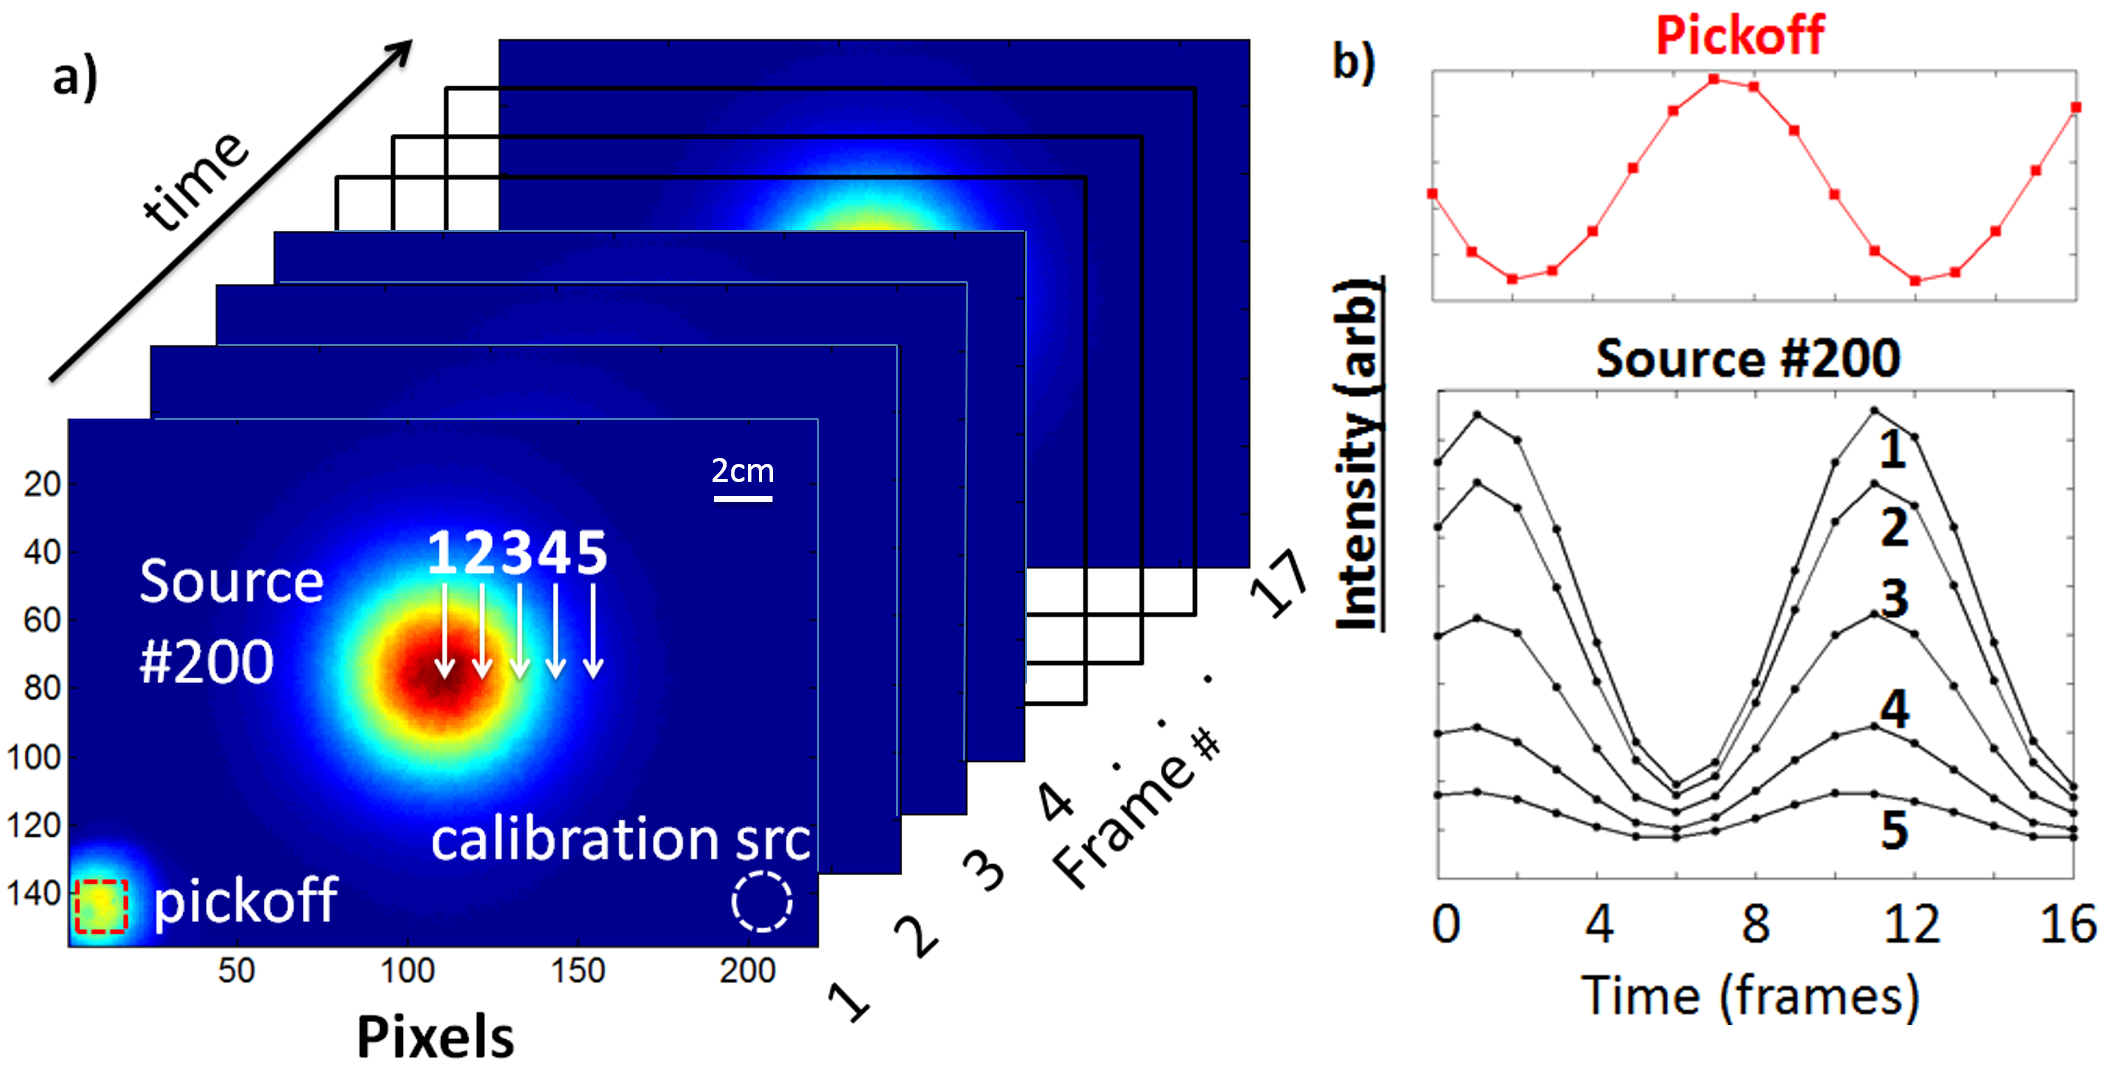
\includegraphics[width=14cm]{./figures/4_Gen3/gen3pp.png}
\caption[Full field time series of light measured by the CCD]{a) Full field time series of light measured by the CCD. The pickoff is in the bottom left corner and measured concurrently. The calibration source is located on the bottom right and taken in series b) (Top) Light signal for a pixel in the pickoff region as a function of time ($17$ frames shown). (bottom) Light signal for different pixels (indicated in (a)) as a function of time. This data is fit to derive $\Phi_{ac}$, and $\theta$.}
\label{fig:gen3pp}
\end{figure}

The Gen3 instrumentation utilizes the pickoff channel shown in Figure~\ref{fig:gen3schem} to correct for changes in  phase due to laser or RF instabilities; this pickoff channel, however, will only account for fluctuations that occur in the source-chain section before the light enters the galvo-switch. This is the reason that we picked off five percent of the light using the $95/5$ optical beam splitter; the $5\%$-light is coupled into a fiber whose output is set in front of the detection window.  Further, a 1-inch thick white delrin is placed in front of the fiber tip and is used as a light diffuser. Importantly, because it is placed in the field-of-view (FOV) of the detection window, this reference signal is obtained concurrently with each source measurement. (Note, an attenuator is added into the pickoff signal pathway so that the light level will be appropriate for the gain and dynamic range of the DOT measurement).
\begin{figure}[t]
\centering
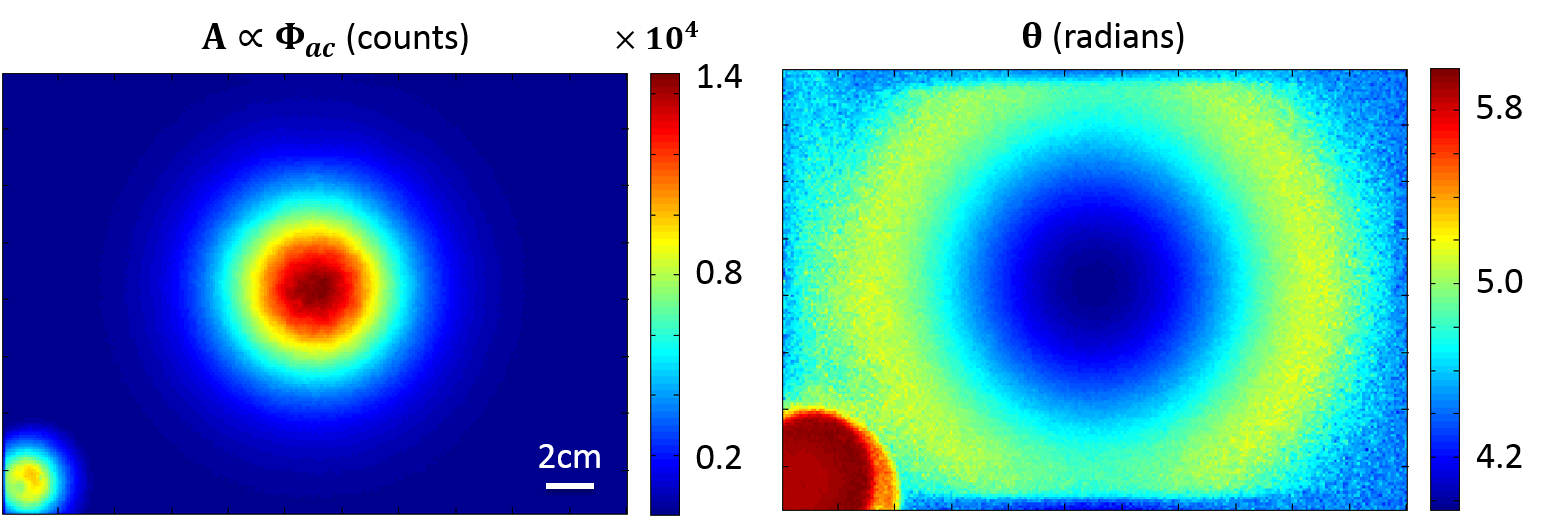
\includegraphics[width=14.5cm]{./figures/4_Gen3/gen3ppdata.png}
\caption[$\Phi_{ac}$ and $\theta$ images after preprocessing]{$\Phi_{ac}$ and $\theta$ images after preprocessing for source $#200$. Every pixel in each image corresponds to a specific source-detector pair with an assigned value for $\Phi_{ac}(\mbf{r_d},\mbf{r_s})$ and $\theta(\mbf{r_d},\mbf{r_s})$}
\label{fig:gen3ppdata}
\end{figure}

Using the pickoff channel signal, preprocessing of the data is implemented in two steps:
\begin{enumerate}[noitemsep]
\item First fit pickoff signal to obtain: $A_{pick}\sin(2\pi f_{cc}t+\theta_{pick})$ (red dotted square shown in Figure~\ref{fig:gen3pp}).
\item Then fit signal of remaining pixels over time to obtain: $A\sin(2\pi f_{cc}t +\theta -\theta_{pick})$.
\end{enumerate}
After these operations, we have obtain $A$ (which is $\propto\Phi_{ac}$) and $\theta$, with the phase offsets from the detection system (i.e., $\theta_{pick}$) corrected. The preprocessed data is shown in Figure~\ref{fig:gen3ppdata}.

A single breast scan enable us to determine $A=C\Phi_{ac}$ and $\theta$ (with some constant source-detector offset $\theta_{offset}$). (See the equations in Section \ref{sec:heterodyne}; $C$ is some unknown coupling constant that, ideally, is expected to be a unique number for each source-detector pair). However, the quantities that we are interested in are $\Phi_{ac}$ and $\theta$ (i.e., without the coupling factor and offset) which are due solely to the optical properties of the breast. By taking a second reference scan with the Intralipid solution alone, we can divide out coupling constants $C$ and subtract out the source offset. For example, from Equation~\ref{eqn:heterodyneresult} we can fit the data to derive the amplitude and phase associated with each source-detector pair for the breast/phantom measurement and for the reference Intralipid measurement. In this case, the needed amplitude ratio and the needed phase shift between sample and reference measurements are readily determined for each source-detector pair, i.e.,
%
\begin{equation}
\frac{A_{breast}}{A_{ref}} = \frac{C\Phi_{ac,breast}}{C\Phi_{ac,ref}} = \frac{\Phi_{ac,breast}}{\Phi_{ac,ref}} \ ;
\end{equation}
\begin{equation}
\Big(\theta_{breast} - \theta_{offset}\Big) -\Big(\theta_{ref} - \theta_{offset}\Big) = \Big(\theta_{breast} - \theta_{ref}\Big) \ .
\end{equation}

This kind of normalization method is critical to implement, but, unfortunately, the approach has limitations, especially since measurements are taken in series. Specifically, since each scan takes 35 minutes, any drifts that occur in the signal (due to temperature changes, movement in the fibers, etc.) will introduce additional errors into the data in addition to the phase that was corrected for with the pickoff signal.

\begin{figure}[t]
\centering
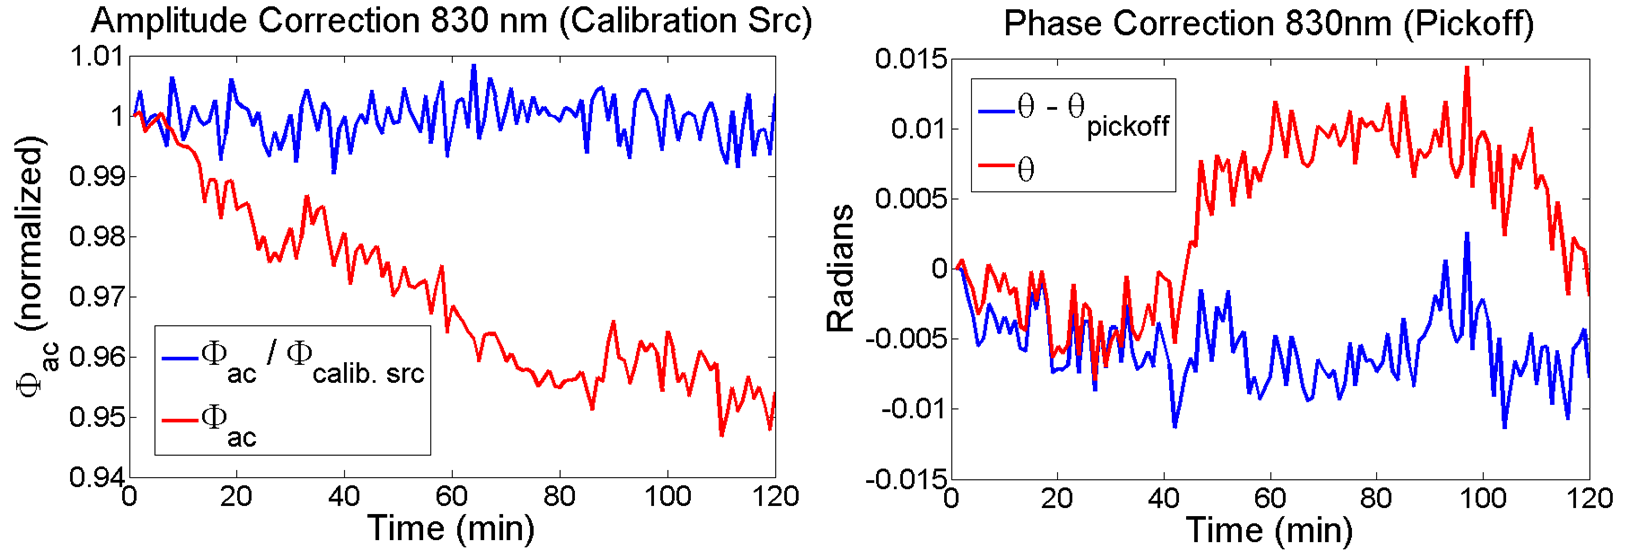
\includegraphics[width=14.5cm]{./figures/4_Gen3/datacorrect.png}
\caption[Time series data showing value of real-time data normalization methods used for the amplitude ($\Phi_{ac}$) and phase ($\theta$)]{Time series data showing value of real-time data normalization methods used for the amplitude ($\Phi_{ac}$, left) and phase ($\theta$, right). The red curve is the uncorrected signal, and blue curve is the corrected curve. The amplitude is corrected using the calibration source and the phase is corrected with the pickoff. This data is with $2\times 2$ pixel binning.}
\label{fig:datacorrect}
\end{figure}

Therefore, in addition to the concurrent reference measurement described in Section~\ref{sec:gen3pp}, the Gen3 instrumentation utilizes one additional source for normalization. This additional source channel is obtained after the galvo-switch (it is the light in the 210th channel; its output is placed far from where the breast signals will be measured as shown in Figure~\ref{fig:srcplatepic} and Figure~\ref{fig:gen3pp}. We refer to this signal as the calibration source. This calibration signal passes through the sample and is taken from another source position fiber; thus, the measurement is not taken concurrently with the other DOT measurements, but rather in series with the DOT measurements. The calibration measurement is typically taken once for every 10 source positions scanned. The advantage of this calibration source is that, unlike the pickoff, the calibration source corrects for changes that might arise due to the galvo or due to the tank and its contents; it is therefore extremely useful for correcting additional relatively-short- and long-term drifts within the system.

Finally, the measurement error $\sigma_{\Phi}$ and $\sigma_{\theta}$ of each pixel is calculated by taking the spatial standard deviation of $5\times 5$ pixels centered on that pixel. This was done using the \textit{stdfilt} function in Matlab over the images in Figure~\ref{fig:gen3ppdata}.

\section{Profilometry}
\label{sec:profilometry}
\subsection{Basics of Profilometry}
To further improve our DOT reconstruction quality, we have built two sets of traditional imaging devices based on the fringe projection profilometry technique. A review describing various implementations of this technique can be found in \cite{Peng2007}. We do not provide a comprehensive discussion of the methodology here, as it is already worked out. Here we simply implement the techniques proposed by Zhang et. al \cite{Zhang2006}, with its emphasis on speed and reduced dependence on the need for projector gamma calibrations (which are time consuming). The details of this section can be skipped with little cost to the overall understanding of my work.
\begin{figure}[b]
\centering
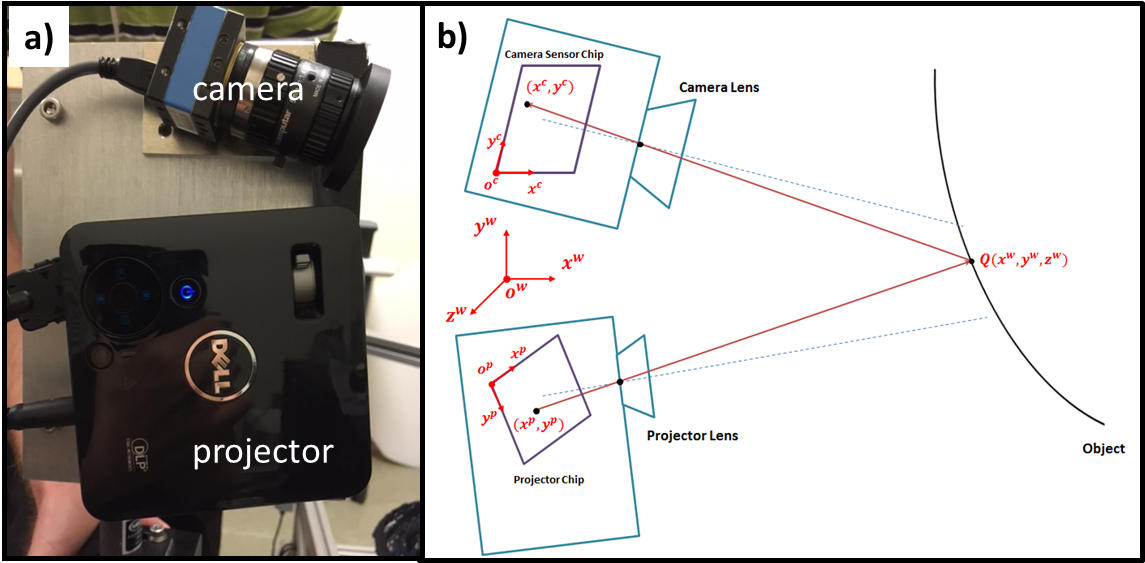
\includegraphics[width=14cm]{./figures/4_Gen3/profcoord.png}
\caption[Schematic of the profilometry setup]{a) Profilometry setup consisting of a camera and portable projector. b) Schematic with the coordinate systems for the camera, projector, and the world or object coordinate.}
\label{fig:profcoord}
\end{figure}
%
\begin{figure}[h]
\centering
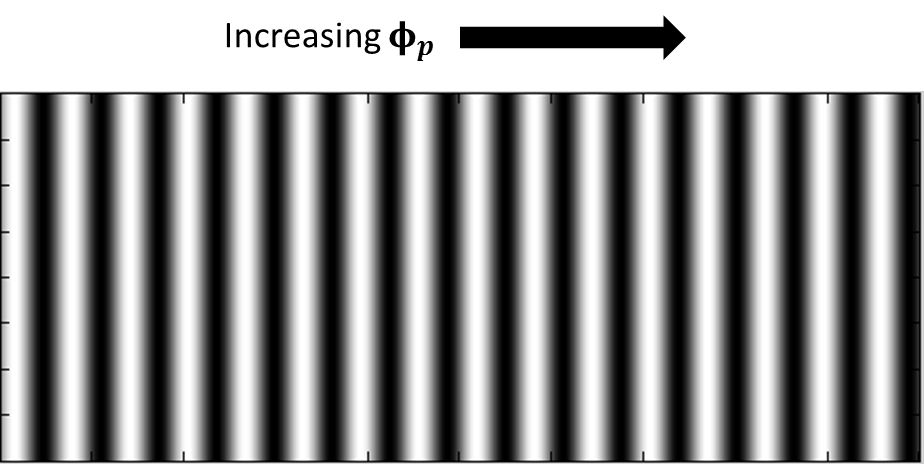
\includegraphics[width=10cm]{./figures/4_Gen3/profphasemap.png}
\caption{Phase map used by the projector based on fringe projection.}
\label{fig:profphasemap}
\end{figure}

Figure~\ref{fig:profcoord} shows a picture of the profilometry device and the corresponding schematic with related coordinate systems for the camera, projector, and the world/object coordinate. The basic steps involved in measuring a 3D surface image with profilometry is the following:
\begin{enumerate}[noitemsep]
\item Project an function, in our case sinusoidal, with increasing phase $\phi_p(x_p)$ along the x-axis of the projector screen onto a flat surface (Figure~\ref{fig:profphasemap}).
\item Image phase map with camera at an angle (see Figure~\ref{fig:profcoord}) with an object placed in the phase map projection. The object will distort the phase $\phi_p(x_p)$ recorded on the camera pixel location $x_c$, $y_c$. Solve for $x_p$ from $\Phi_p(x_p)$.
\item Convert ($x_c, y_c, x_p$) to the world spatial coordinate ($x_w,y_w,z_w$) (calibrations needed) which gives us our surface 3D map.
\end{enumerate}

In practice, a sinusoidal fringe projection (as shown in Figure~\ref{fig:profphasemap}) where each column on the projector screen have the same value of $\phi_p(x_p)$. Objects that are moved into the field of view of this phase map will shift the columns of the fringe pattern (note that the shift direction depends on the position of the camera relative to the projector). The magnitude of this shift will contain information in the height of the object as bigger objects will result in bigger shifts in the fringe patterns. Alternatively, the projector can be thought of defining a plane with a particular phase value, while the pixel of the CCD defines a line that intersects the plane from its point-of-view. The place where the line intersect with the plane will define a point in space from which we get our surface information.

Thus one only needs to record the the value of $\phi_p(x_p)$ at a given camera pixel at ($x_c,y_c$), solve for $x_p$ from $\phi_p(x_p)$ (which is known), then map coordinates ($x_c, y_c, x_p$) to the world spatial coordinate ($x_w,y_w,z_w$). Implementing the three steps above for fringe profilometry we have:

\\
\noindent
\textbf{Step 1:} Project fringe patterns onto the object we (Figure~\ref{fig:profunwrap}) (a):
\begin{eqnarray}
\label{eqn:projfringe}
\phi_p(x_p,y_p)& = & 2\pi f_p x_p \label{eqn:x_p} \ ; \\
P_{p,1}(x_p,y_p) & = & \frac{P_{p,max}}{2} \frac{P_{p,max}}{2}\cos(\phi_p(x_p,y_p)-2\pi/3)\notag \ ; \\
P_{p,2}(x_p,y_p) & = & \frac{P_{p,max}}{2} \frac{P_{p,max}}{2}\cos(\phi_p(x_p,y_p))\notag \ ; \\
P_{p,3}(x_p,y_p) & = & \frac{P_{p,max}}{2} \frac{P_{p,max}}{2}\cos(\phi_p(x_p,y_p)+2\pi/3) \ .
\end{eqnarray}

Here $P_{max}$ is the maximum intensity of the projector and $\phi_p(x_p,y_p)=\phi_p(x)$ is the encoded phase on the projector. $f_p$ is the spatial frequency of the fringe and scales with the change in height variation that is expected in the objects we would like to measure and is determined experimentally. Subscript $p$ denotes that we are in the projector coordinates (more on this later). In the above case we made $\phi_p(x_p,y_p)=\phi_p(x)$ such that each column of the projector chip is encoded with one phase value. Three projections are made with offset phase so that we can solve for the phase when we measure the fringe patterns with the camera. Solving Equation~\ref{eqn:x_p} gives us $x_p=\phi_p/(2\pi f_p)$.
\begin{figure}[ph]
\centering
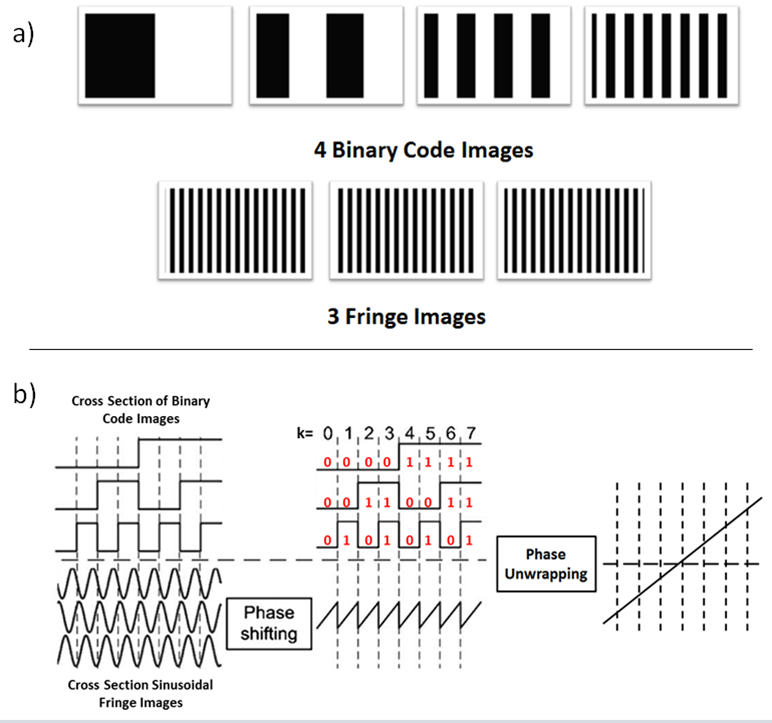
\includegraphics[width=10cm]{./figures/4_Gen3/profunwrap.png}
\caption[Fringe projection unwrapping scheme]{a) Binary and fringe projections from the projector. b) Unwrapping scheme proposed by Zhang et al. that uses the binary information encoded by the binary projections.}
\label{fig:profunwrap}
\vspace{5mm}
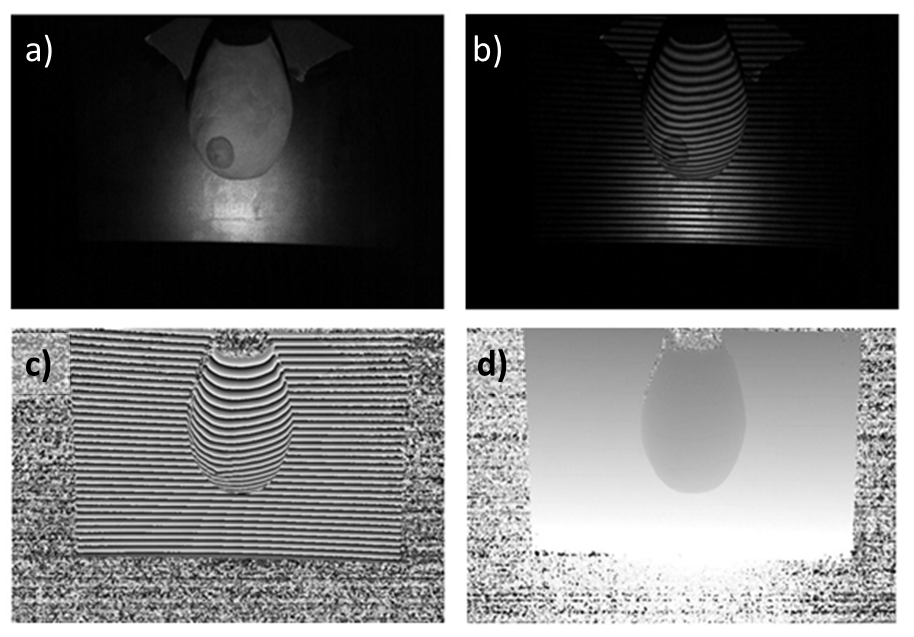
\includegraphics[width=13cm]{./figures/4_Gen3/proffringe.png}
\caption[Profilometry projections]{a) Object image, b) fringe patterns projected onto object, c) phase image, and d) unwrapped phase image.}
\label{fig:proffringe}
\end{figure}


\noindent
\textbf{Step 2:} Measure fringe patterns with camera and solve for the distorted phase due to the object.
\begin{eqnarray}
\label{eqn:fringe}
M_{c,1}(x_c,y_c) & = & M_{c,dc}(x_c,y_c)+M_{c,ac}(x_c,y_c)\cos(\phi_c(x_c,y_c)-2\pi/3)\notag \\
M_{c,2}(x_c,y_c) & = & M_{c,dc}(x_c,y_c)+M_{c,ac}(x_c,y_c)\cos(\phi_c(x_c,y_c))\notag\\
M_{c,3}(x_c,y_c) & = & M_{c,dc}(x_c,y_c)+M_{c,ac}(x_c,y_c)\cos(\phi_c(x_c,y_c)+2\pi/3) \\
\phi_c(x_c,y_c)  & = &\arctan\big(\frac{\sqrt{3}(P_{c,1}(x_c,y_c)-P_{c,3}(x_c,y_c)}{2P_{c,2}(x_c,y_c)-P_{c,3}(x_c,y_c)}\big) \label{eqn:phi_c}
\end{eqnarray}
\noindent
where $M_{c,dc}$ is the measured average intensity, $P_{c,dc}$ is the modulation amplitude and $\phi_c$ is the phase value we want to solve for. The subscript $c$ denotes the camera reference. Equation~\ref{eqn:phi_c} can be used to solve for $\phi_c$. Fortunately, since we chose to increase the phase map along one axis, aligning the camera and projector parallel to this axis allow the approximation that $\phi_c=\phi_p$. Before we can solve for our surface map, we need to unwrap as sinusoidal projections repeat in phase over [$-\pi, \pi$]:
\begin{equation}
\Phi_c(x_c,y_c)= \phi_c(x_c,y_c)+2\pi\cdot k(x_c,y_c)
\end{equation}
Here $k$ is called the fringe number. The value of $k$ cannot be solved without additional information. The value of $k$ can be encoded into our camera by projecting an additional set of images to encode binary information spatially \cite{Zhang2006}. A schematic diagram of the projections used and the binary encoding method is shown in Figure~\ref{fig:profunwrap}(a). Using a set of four binary code images encode each camera pixel with 4-bit information corresponding to a value of k. An example is shown in Figure~\ref{fig:profunwrap}(b) for a 3-bit case. Implementing these steps, we are able to unwrap the phase as shown in Figure~\ref{fig:proffringe}(b).


\noindent
\textbf{Step 3:} Convert ($x_c,y_c,x_p$) $\rightarrow$ ($x_w,y_w,z_w$)
At this point we have $x_c,y_c,$ and $x_p$. We can convert these values to a point in space with the following equations:
\begin{align}
x_c &= P_{c,11}x_w + P_{c,12}y_w + P_{c,13}z_w + P_{c,14} \notag \ ; \\
y_c &= P_{c,21}x_w + P_{c,22}y_w + P_{c,23}z_w + P_{c,24} \notag \ ; \\
x_p &= P_{p,11}x_w + P_{p,12}y_w + P_{p,13}z_w + P_{p,14} \label{eqn:profcoordcal} \ ,
\end{align}
where $P_c=A_{i,c}[R_c,t_c]$ and $P_p=A_{i,p}[R_p,t_p]$ where $A_i$ is the intrinsic parameter matrix (which take into account the focal length and skew), $R$ is the rotational matrix, and $t$ is the translational matrix. Solving Equation~\ref{eqn:profcoordcal} gives us ($x_w,y_w,z_w$) for every ($x_c,y_c,x_p$) which, in turn, give our 3D surface map! I will not go into details of the calibration method to find the values of $A_i,R,$ and $t$ for the camera and projector, but I refer interested reader to \cite{Peng2007,Zhang2010,Gorthi2010,Geng2011}.

\subsection{Profilometry Setup and Breast Shape Measurement}
The profilometry setup used in the Gen3 system is shown in Figure~\ref{fig:profcoord}(a). The setup consists of a projector (M110, Dell) and a small CMOS camera (DMK 72AUC02, The Imaging Source)  with a $5~\rm{mm}$ lens (H0514-MP2, The Imaging Source) mounted on a custom aluminum block. Once the projector and camera positions are fixed relative to each other, the coordinate and height calibrations are made. Two profilometry setups are used in the Gen3 system and mounted on the sides of the imaging tank as shown in Figure~\ref{fig:proftank}.
\begin{figure}[ph]
\centering
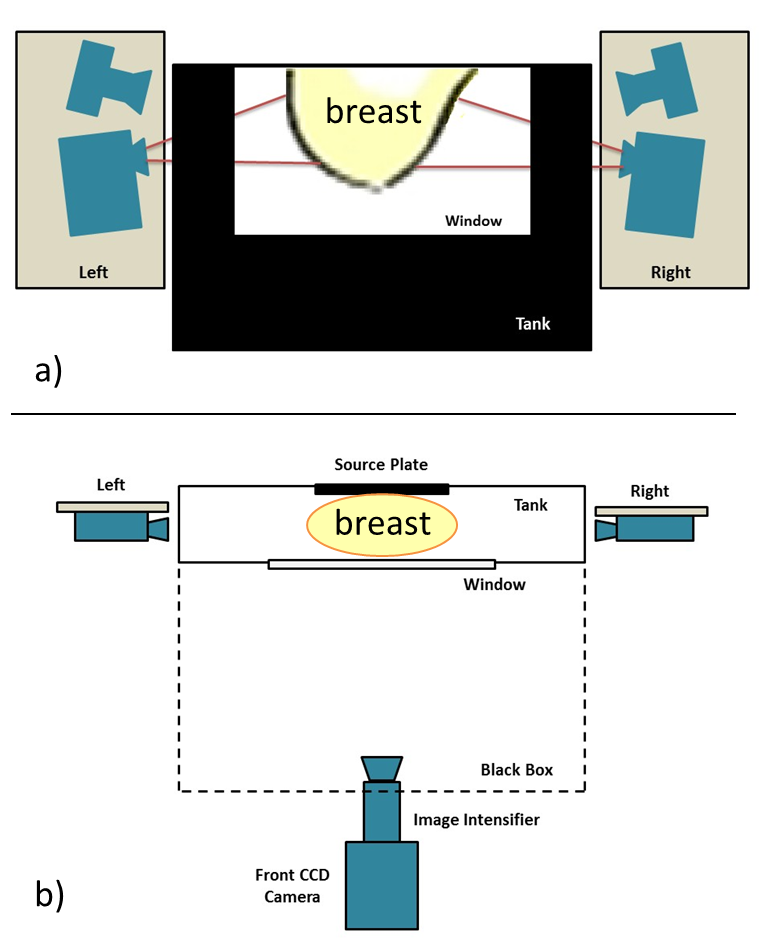
\includegraphics[width=10cm]{./figures/4_Gen3/proftank.png}
\caption[Schematic of profilometry system relative to Gen3 imager]{a) Front view of profilometry system from Gen3 CCD perspective b) top view.}
\label{fig:proftank}
\vspace{5mm}
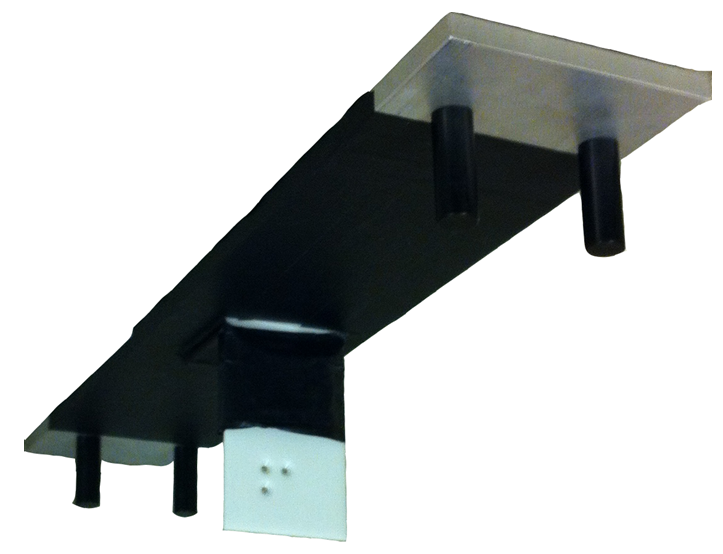
\includegraphics[width=7cm]{./figures/4_Gen3/profcalib.png}
\caption[Photograph of the profilometry positioning calibration target]{Photograph of the profilometry positioning calibration target use to map the images from the profilometry sets and the Gen3 CCD onto the same space. The white plate, with three holes, hangs down in the tank and is used to align the rotational and translational position of the profilometry 3D surface images relative to one another.}
\label{fig:profcalib}
\end{figure}

After the breast is inserted into the imaging tank, profilometry images are taken from the sides. Figure~\ref{fig:profdata} shows data from a human subject. In most cases, the area covered by the two profilometry sets is not large enough to obtain a 3D surface image of the whole breast. Thus, the bottom side of the breast must be generated with a 3D surface fit based on data in Figure~\ref{fig:profdata}(a) and (b). To improve the accuracy of this bottom surface fit, a sagittal image from the CCD is acquired in addition to the profilometry data (see Figure~\ref{fig:profdata}(c)). The saggital image is used to determine outer edge of the breast shown by a red line, which, in turn, is used to aid the bottom surface fit.  
\begin{figure}[!htp]
\centering
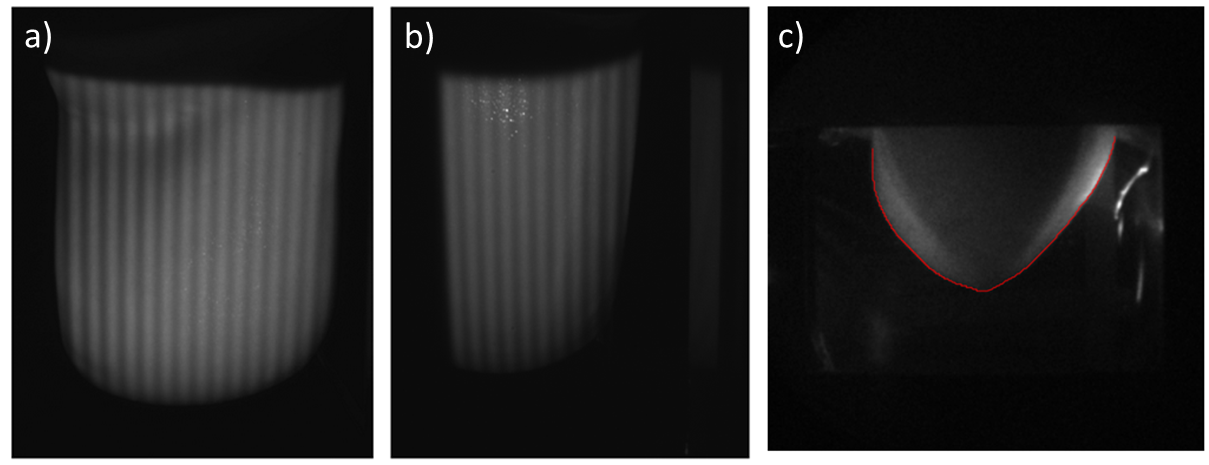
\includegraphics[width=14cm]{./figures/4_Gen3/profdata.png}
\caption[Examples of profilometry measurements of the breast]{a) Fringe pattern projected on the breast (left side of tank), b) fringe pattern on right side of tank, and c) sagittal view of breast from front CCD. Red line shows outer edge of breast traced by hand.}
\label{fig:profdata}
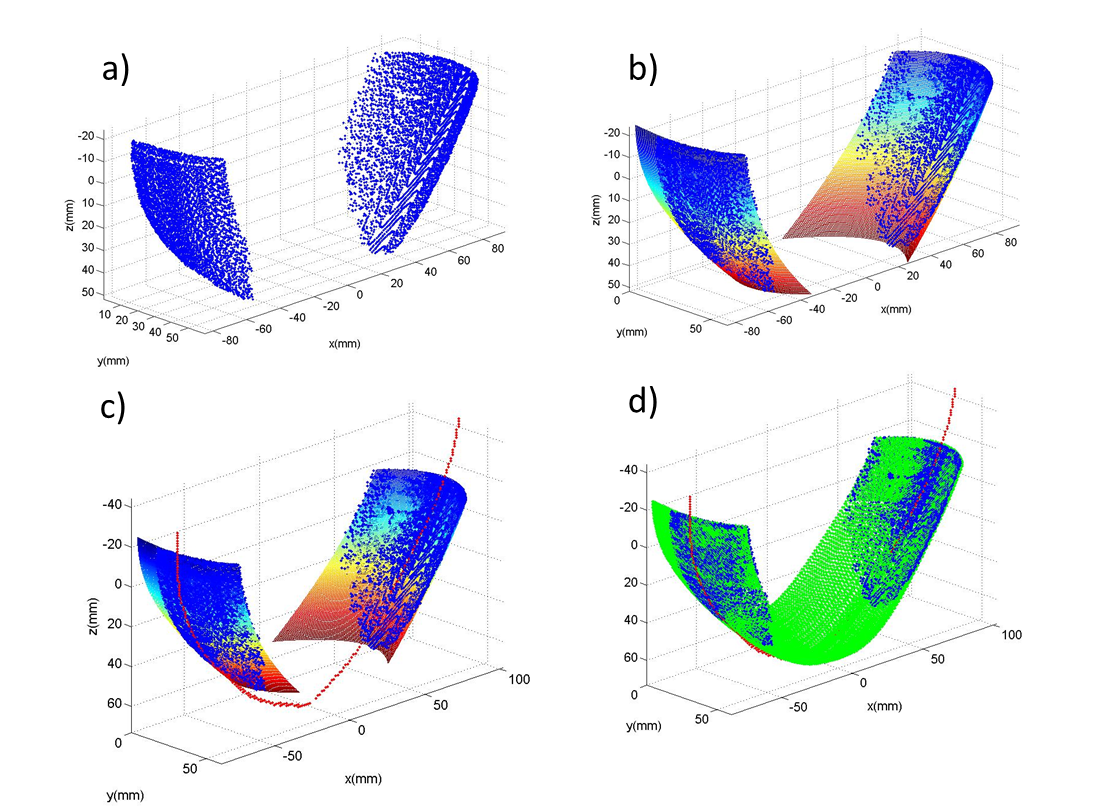
\includegraphics[width=14.5cm]{./figures/4_Gen3/proffit.png}
\caption[Profilometry data fits for 3D surface]{ a) 3D point cloud generated by fringe profilometry b)  surface fit of 3D point cloud c) line trace (red) from front CCD camera scaled and translated to match side surfaces d) 3D surface fit of whole breast generated from fringe profilometry data and front image trace.}
\label{fig:proffit}
\end{figure}

The relative positions of the two profilometry surfaces are linked together with one additional measurement obtained using a positioning calibration target shown in Figure~\ref{fig:profcalib}. The three holes in the target helps with the profilometry sets, i.e., helps to align their position and rotation relative to each other. The target is designed to always fit into the tank in the same position; this feature helps us match the profilometry sets to the Gen3 CCD (and the red line from the sagittal image).

To generate the 3D surface image, the two surface point clouds generated by the profilometry sets are combined with the outer trace (red line) of the breast image from the CCD to derive the surface on the bottom side of the breast that was not illuminated by the profilometry projectors. The resulting 3D surface fit is then used to generate a tetrahedral volume mesh to be used in the DOT image reconstruction.
%
\section{Clinical Software}
\label{sec:clinicalui}
The software for the Gen3 device was written in Labview. Two sets of software were written to run measurements on the Gen3 device. The Experimental Software permits an advanced user to fully control the Gen3 device hardware settings and measurement sequences. This Experimental Software is also used to generate a configuration file used in experiments where various CCD settings can be set and saved for use on the Clinical Panel.

The Clinical Software was written with our clinical coordinators in mind (see Figs.~\ref{fig:Clinical1}). Five modules in sequence take the user from tasks that organize the output files to tasks that choose the source and wavelength configuration, tasks that optimize the detection gain and output light levels, and finally to screens that allow the user to start the measurement sequence and see its progress. For detailed description of the software I refer the user to Appendix A.

\section{Instrument Characterization}
\subsection{Spectroscopy}
Although the data used in DOT reconstructions are normalized to measure relative changes in optical properties (see Section~\ref{sec:gen3pp}), one way to test the imaging system is to compare a measurements that extract absolute values of $\mua$ and $\musp$ in a Intralipid solution to slab theory predictions. In particular, this scheme enable us to evaluate the data quality of the frequency-Domain (FD) detection capabilities of the Gen3 imager. Figure~\ref{fig:slabfit} shows data from the FD transmission data that has been preprocessed;  comparison to a slab solution model is also shown. The light was from a source near the center of the detection lens. Figure~\ref{fig:slabfit} shows the slab solution fit for $\mua$ and $\musp$ of a homogeneous Intralipid solution; the results exhibit reasonable agreement with expected values.
%
\begin{figure}
\centering
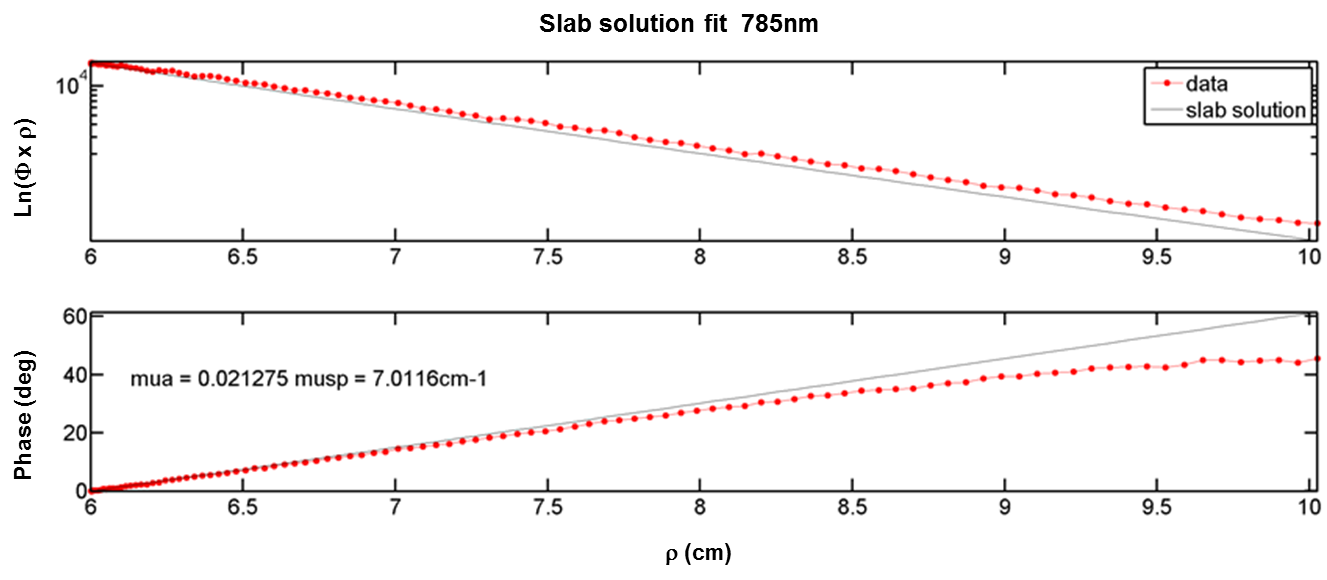
\includegraphics[width=14.5cm]{./figures/4_Gen3/slabfit.png}
\caption[Slab solution fit to frequency-domain data]{Comparison of $\ln (\Phi_{ac}\times\rho)$ and Phase ($\theta$) vs $\rho$ of the Gen3 data from a line of pixels and the analytical slab solution fit to the data for $\mua$ and $\musp$. Expected values were $\mua= 0.021 cm^{-1}$ and $\musp=8cm^{-1}$}
\label{fig:slabfit}
\end{figure}
\floatbarrier
\begin{figure}[hp]
\centering
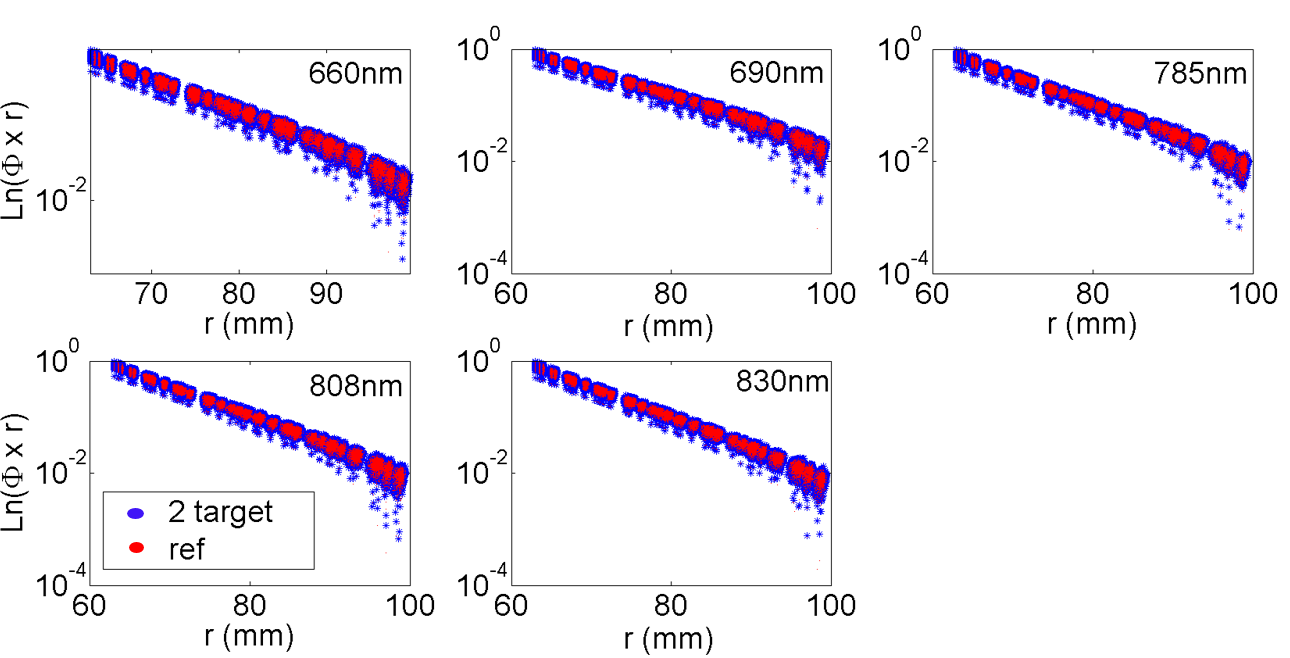
\includegraphics[width=14.5cm]{./figures/4_Gen3/srcamp.png}
\caption[$\ln (\Phi_{ac}\times r)$ vs $r$ plots for all source-detector pairs of the Gen3 imager]{$\ln (\Phi_{ac}\times r)$ vs $r$ plot for all $209$ sources at all $5$ wavelengths. The tank thickness is $63~\rm{mm}$. Usually, the data usage is cut off around $r=85~\rm{mm}$ where noise starts to become significant. Repeatability between target and reference data (blue vs red) as well as linearity vs $r$ provide criteria by which we can judge data quality.}
\label{fig:srcamp}
\vspace{10mm}
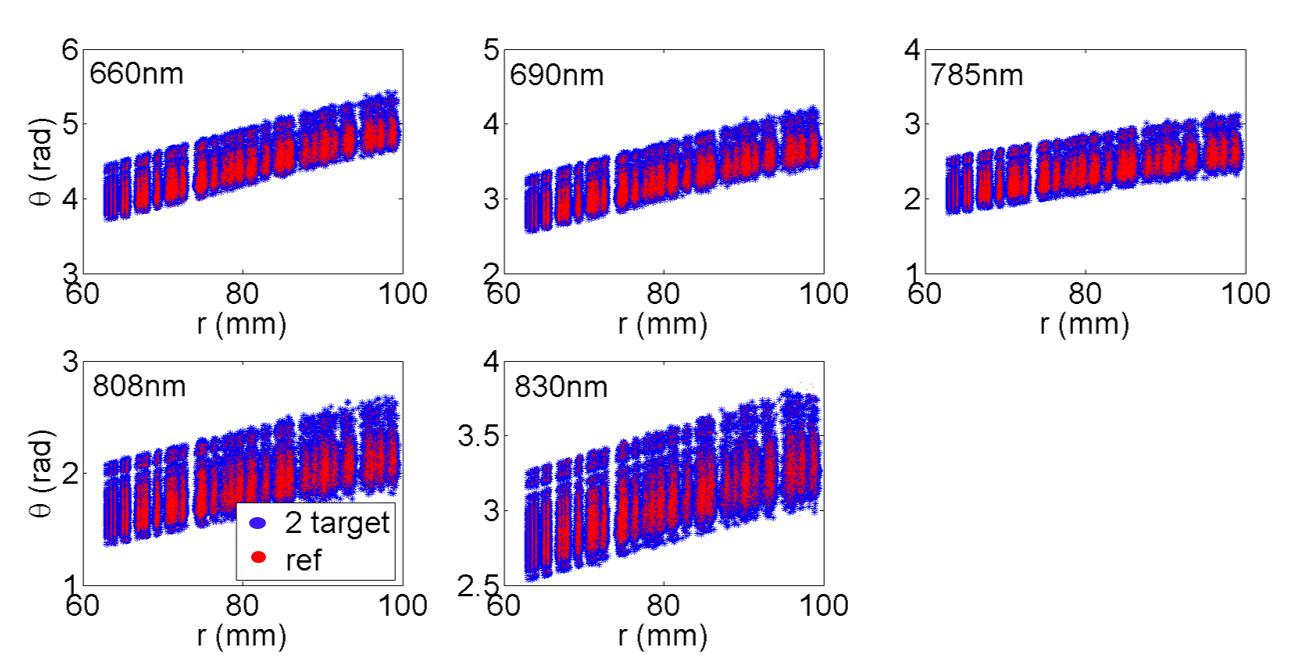
\includegraphics[width=14.5cm]{./figures/4_Gen3/srcphase.png}
\caption[$\theta_{ac}$ vs $r$ plots for all sources and detectors of the Gen3 imager]{$\theta_{ac}$ vs $r$ plot for the same data set in Figure \ref{fig:srcamp}. The distribution of values for $\theta(63~\rm{mm})$ is due (in part) to variations of the source fiber length, i.e., since the fibers were assembled by hand (see Section~\ref{sec:sources})}
\label{fig:srcphase}
\end{figure}
\begin{figure}[t]
\centering
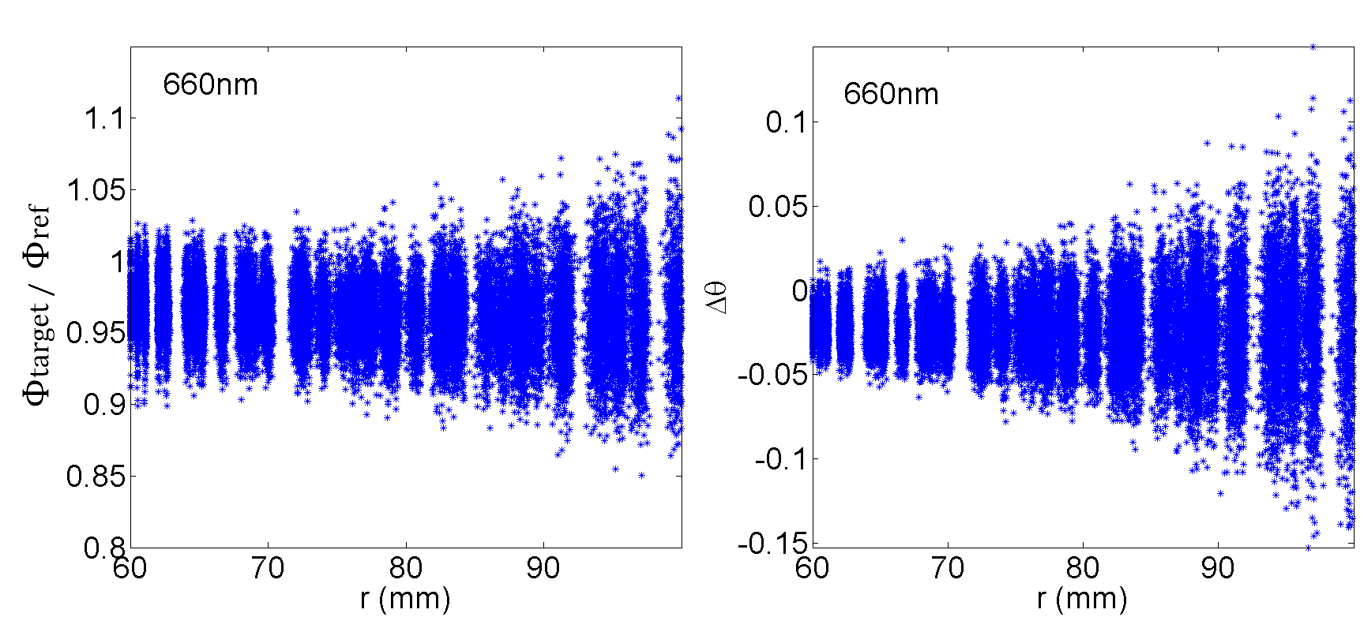
\includegraphics[width=14.5cm]{./figures/4_Gen3/dPhidphase.png}
\caption[Difference data of $\Phi$ and $\theta$]{Plot of $\Phi_{target}/\Phi_{ref}$ (left) where the two target scan in Figure~\ref{fig:srcamp} is divided by the reference scan (normalized) for each source detector pair. $\Delta\theta=\theta_{target}-\theta_{ref}$ (right, radians) where the two target scan in Figure~\ref{fig:srcphase} for the two target and reference measurements (at $660~\rm{nm}$) for all source detector pairs. The width of the differences is used to derive a criteria for how large a source-detector separation ($\sim80mm$) we should use before noise becomes important.}
\label{fig:dPhidphase}
\end{figure}
\floatbarrier

In general, determination of the absolute value of $\mua$ and $\musp$ in this way cannot take advantage of all source locations, e.g., due to vignetting and barreling that occurs when light travels too far from the center of the detection lens. However, when normalized with a reference measurement as described in Section~\ref{sec:gen3pp}, then optical property changes can be measured using all source-detector pairs. This is because one can account for the pathologies associated with each source-detector. 

To get a sense of these deviations in the data (in absolute terms), in Figure \ref{fig:srcamp} and \ref{fig:srcphase} we plot the preprocessed data from all the detectors (CCD pixels) for every source and every wavelength. The two data sets are derived from tissue phantom (red: two target--see next section) and a Intralipid reference measurements (blue), respectively. This particular dataset should overlap as the only differences in the measurement are due to two small perturbations. Figure~\ref{fig:dPhidphase} shows plots the normalized amplitude, $\Phi_{target}/\Phi_{ref}$, and the phase shift $\Delta\theta =\theta_{target}-\theta_{ref}$ for $660$ nm. Thus the quality of the reference normalization can be determined the general agreement in the data points. The SNR of the signal also determines how large $r$ can be before the fluence rate ($\ln (\Phi_{ac}\times r)$) and $\theta$ begin to lose linearity (e.g., around $85~\rm{mm}$).
\floatbarrier
\subsection{Targets for Imaging Experiments}
The frequency-domain capabilities of the Gen3 imager make it easier to reconstruct both absorption and scattering contrast properties. This capability was relatively weak in the Gen2 system. As a result we developed new kinds of targets appropriate for frequency domain experiments. The targets we use are typically hollow containers filled with contrast media for imaging. Our old targets were made from translucent cylinder plastic containers ($1.5~\rm{cm}$ in diameter and 1.5 cm in height) connected to thin Tygon tubing for loading contrast media. For these targets, the perturbation to absorption was low (Figure~\ref{fig:targettrans}(b), but the target material contributed significant phase contrast (Figure~\ref{fig:targettrans}(c). In fact, we can more readily detect these phase contrast signals with the new (Gen3) frequency domain system.
%
\begin{figure}
\centering
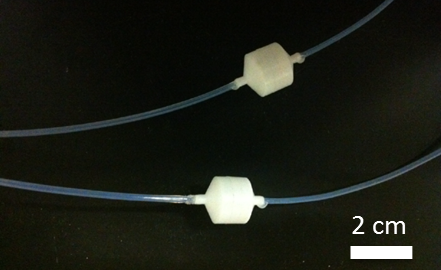
\includegraphics[width=7cm]{./figures/4_Gen3/targetpic.png}
\caption[Photograph of custom targets used for imaging liquid phantoms.]{Photograph of custom targets used for imaging liquid phantoms. The targets are made of white delrin with $16$ mm diameter and $1$ mm thick walls. The targets are attached to a thin nylon tubing and sealed with silicone gel. The targets are hung vertically and shaped so that air bubbles freely escape.}
\label{fig:targetpic}
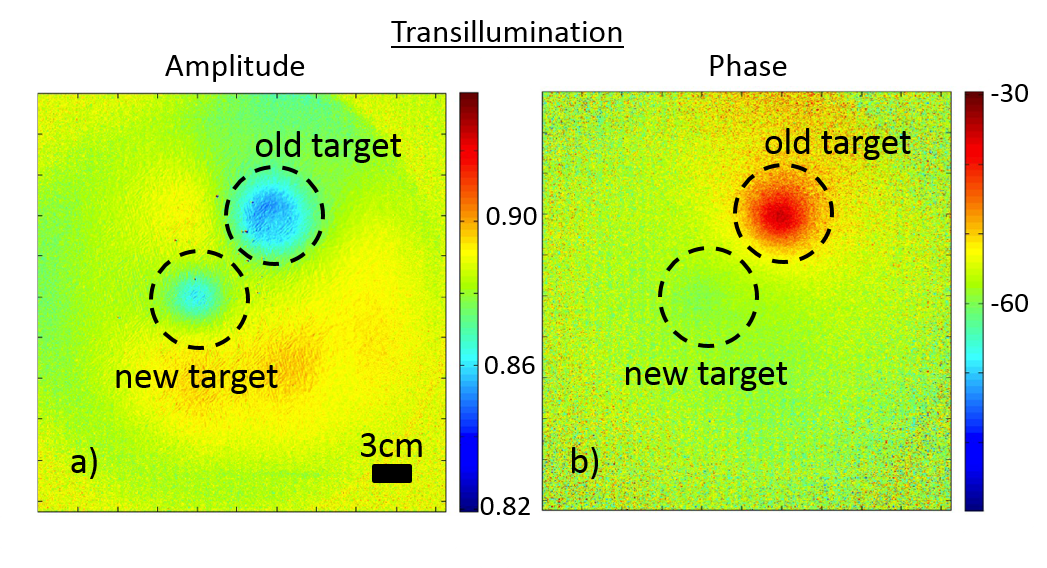
\includegraphics[width=14.5cm]{./figures/4_Gen3/targettrans.png}
\caption[Transillumination images of Delrin target]{a) Transillumination images of Delrin target (bottom left) and a typical translucent plastic target. White delrin is a good choice as it has scattering and absorption properties similar to Intralipid. (left) Transillumination amplitude data of Intralipid filled targets in the background fluid (normalized intensity). (Right) Transillumination phase data (degrees).}
\label{fig:targettrans}
\end{figure}
%
Several translucent or white materials were tested with the transillumination experiment shown in Figure~\ref{fig:targettrans}. Targets filled with the background Intralipid ($\mua=0.041 cm^{-1}$, $\musp=8 cm^{-1}$) were suspended inside the reference solution in a tank (the same tank used in Chapter 3) and the amplitude and phase data were collected. Importantly, we found that white Delrin with thin PTFE tubing (microbore, Cole Palmer) introduced the lowest amplitude and phase contrast artifacts (Figure~\ref{fig:targetpic}).
\floatbarrier
\section{Simulations}
The data from the Gen3 imager was reconstructed using a software suite called TOAST++ (Time-resolved Optical Absorption Scattering Tomography) \cite{Schweiger2014}. TOAST employs FEM for the forward problem and Newton-type (Gauss-Newton, Levenberg-Marquardt, etc.) or gradient-type (Conjugate Gradient) methods for the inverse problem. Simulation results based on the Gen3 imager configuration (and related to actual experiments performed with the Gen3 imager) are presented in this section.

Simulations are valuable. They permit testing of constraints for the geometry, source-detector pair arrangement, and data type of a particular imaging system (e.g., Gen3). Furthermore, limitations of the reconstruction method can be tested, and control parameters (e.g., regularization parameters) can be adjusted with repeated reconstructions to reduce and optimize the parameter space for ultimate experiments with real data.

\subsection{2D Reconstructions of Simulated Data}
\label{sec:2Dsim}
We carried out a set of simulated 2D reconstructions on noiseless data.  These test-studies enabled us to confirm that we obtain expected results in situations wherein all aspects of the problem are fully under control and the target medium is fully understood. Although significant differences can arise between 2D and 3D data, as well as for reconstructing with and without noise, the 2D simulations we carry out significantly reduce the scale of the problem and enable us to explore limitations of the reconstruction methods within a short period of time (i.e., on the order of minutes per reconstruction in 2D, rather than hours in 3D).

Figure~\ref{fig:2Dsim} shows the target medium from which simulated data was generated, as well as the 2D reconstruction of the absorption and scattering targets. The reconstructed area is a $80\times 20$ pixel ($3$ mm/pixel) with $\mua$ and $\musp$ inclusions that are $1.8$ cm in diameter (Figure~\ref{fig:2Dsim}(a)). The first column shows the true absorption contrast in the target medium and the second column shows the true scattering contrast in the target medium. The reconstruction of these inclusions is shown in Figure~\ref{fig:2Dsim}(b).
\begin{figure}[t]
\begin{center}
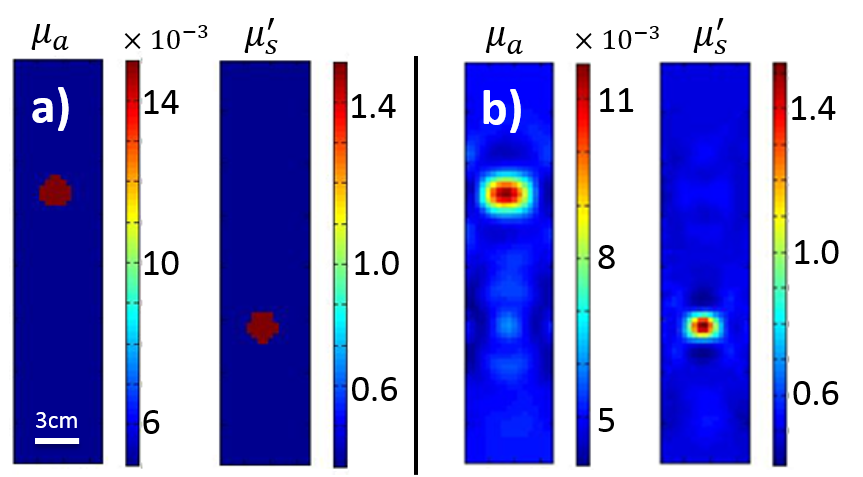
\includegraphics[width=12cm]{./figures/4_Gen3/2Dsim.png}
\caption[Simultaneous 2D reconstruction of $\mua$ and $\musp$ with 3:1 contrast targets for both based on simulated data]{Simultaneous 2D reconstruction of $\mua$ and $\musp$ with 3:1 contrast targets for both based on simulated data. a) Exact image of the target absorption $\mua=0.015~\rm{mm}^{-1}$ (left) and scattering $\musp=1.5~\rm{mm}^{-1}$ (right) with target background $\mua=0.005~\rm{mm}^{-1},~\musp=0.5~\rm{mm}^{-1}$ b) Gauss-Newton reconstruction of $\mua,~\musp$ from forward data obtained with this simulated phantom with uniform regularization and scaling of both scattering and absorption heterogeneities to their average/background.}
\label{fig:2Dsim}
\end{center}
\end{figure}

Notice that the reconstructed absorption target in the simulation is larger than the scattering target by about a factor of $\sim 50\%$. Further, the scattering target is close to the same size as the test inclusion, but the absorption target is not. Also, a very small amount of crosstalk is evident wherein the scattering inclusion shows up in the absorption reconstruction. We can partially understand the size discrepancy between the absorption and scattering inclusions by considering the sensitivity plots shown in Figure~\ref{fig:2Djacob}. The sensitivity plots show the spatial sensitivity of the measured amplitude ($\Phi_{ac}$) and phase ($\theta$) data with respect to $\mua$ and $\musp$ for a particular source-detector pair. The plots in Figure~\ref{fig:2Djacob} show that $\mua$ sensitivity spans over a larger spatial area compared to scattering; this observation helps to explain the larger size of the absorbing target in the reconstruction. Conversely, the $\musp$ sensitivity is spatially smaller and more localized than absorption, which presumably helps to produce a more spatially defined target (i.e., compared to absorption) in the reconstructions. We will return to describe a regularization strategy that can cope with this observation of asymmetry between absorption and scattering reconstruction.

\begin{figure}[t]
\begin{center}
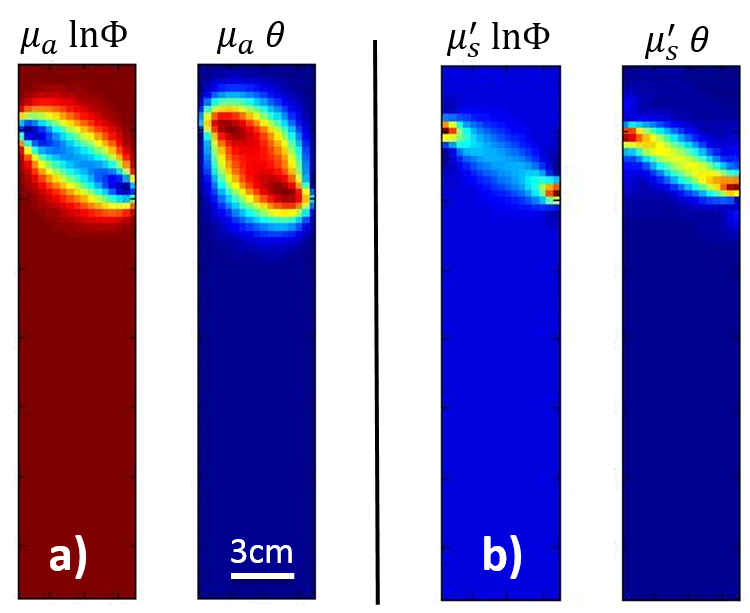
\includegraphics[width=10cm]{./figures/4_Gen3/2Djacob.png}
\caption[Plot of the sensitivity regions (Jacobian) for a source-detector pair]{Plot of the sensitivity regions (Jacobian) for a source-detector pair. a) The two images are the sensitivity of $\ln \Phi_{ac}$ and $\theta$ to changes in $\mua$; b) the two images are the sensitivity of $\ln \Phi_{ac}$ and $\theta$ to changes in $\musp$. Notice, $\ln \Phi_{ac}$ and $\theta$ have a broader area of sensitivity to changes in the absorption compared to changes in scattering.}
\end{center}
\end{figure}

Before moving to the regularization strategies and tests, I describe one more technical effect that we noticed about these systems from the simulations. This effect concerns the trade-off between resolution/contrast and field-of-view angle. In our experimental data, for the typical image slabs, the transverse distance that we can access above the noise level is approximately $8.5~\rm{cm}$. This transverse distance (and the slab separation) defines a maximum field-of-view angle for the data set. In the simulation studies, since we have no noise, we were able to carry out reconstructions for different transverse distances (at fixed slab thickness) and compare the reconstructions. Figure~\ref{fig:2Dfanbeam} shows reconstructions wherein the transverse distance is set to be a)$\mbf{r}=8$ and b) $\mbf{r}=10~\rm{cm}$. As expected the larger $\mbf{r}$ improves our resolution overall, but mostly the improvements occur for the absorption heterogeneity. Therefore, this small but focused 2D simulation investigation informs us that substantial resolution gains can be made with our apparatus, if the signal-to-noise ratio (SNR) of our system can be improved, i.e., if we can make collect data at larger source-detector separations.
\begin{figure}[t]
\begin{center}
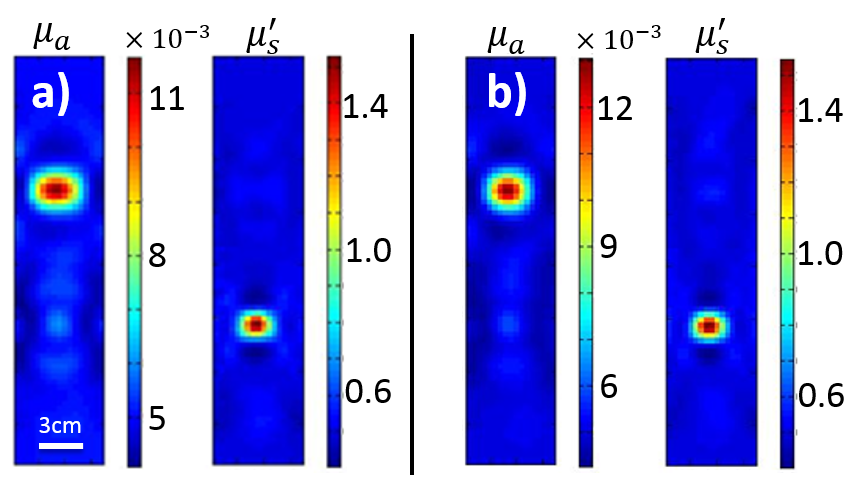
\includegraphics[width=13cm]{./figures/4_Gen3/2Dfanbeam.png}
\caption[Comparison of simulation reconstructions with different maximum transverse distances]{a) Same reconstruction as Figure~\ref{fig:2Dsim}(b) where the maximum transverse distance (along the detection plane) for data taking is $\mbf{r}=8~\rm{cm}$. b) Reconstruction with maximum transverse distance set to $\mbf{r}=10~\rm{cm}$. Larger $\mbf{r}$ produces better resolution in the reconstruction.}
\label{fig:2Dfanbeam}
\end{center}
\end{figure}

We now return to the regularization issue. To our knowledge, researchers in the DOT community have treated absorption and scattering on the same footing. However, we have shown that the absorption target reconstruction is worse than the scattering target reconstruction (i.e., with sensitivity curves and with the reconstructions of simulated data). This observation suggests that it might be better to apply separate regularization for each of these parameters. We explored this approach using Total Variation (TV) regularization, which is largely oriented towards the spatial gradient of the optical properties and thus has the effect of conserving edge shapes. Total Variation (TV) regularization was used here, because we found it to have an improved effect on the resolution of the reconstructions of simulated data. Figure~\ref{fig:2Dtvreg} shows the TV regularization applied to our previous reconstruction with various hyperparameters $\Lamda$ and the TV parameter $\beta$ (see Section~\ref{sec:reg} in Chapter 2). By varying the parameters and then carrying out a corresponding reconstruction, it was determined that the parameters $\Lambda=1\times10^{-4}$, $\beta=1\times10^{-3}$ for $\mua$, and $\Lambda=1\times10^{-3}$, $\beta=1\times10^{-2}$ for $\musp$, gave the best fidelity for absorption at the cost of some scattering contrast. This choice of regularization also brought the size of the reconstructed absorption and scattering targets into the same range, which is also an improvement.
%
\begin{figure}[h]
\begin{center}
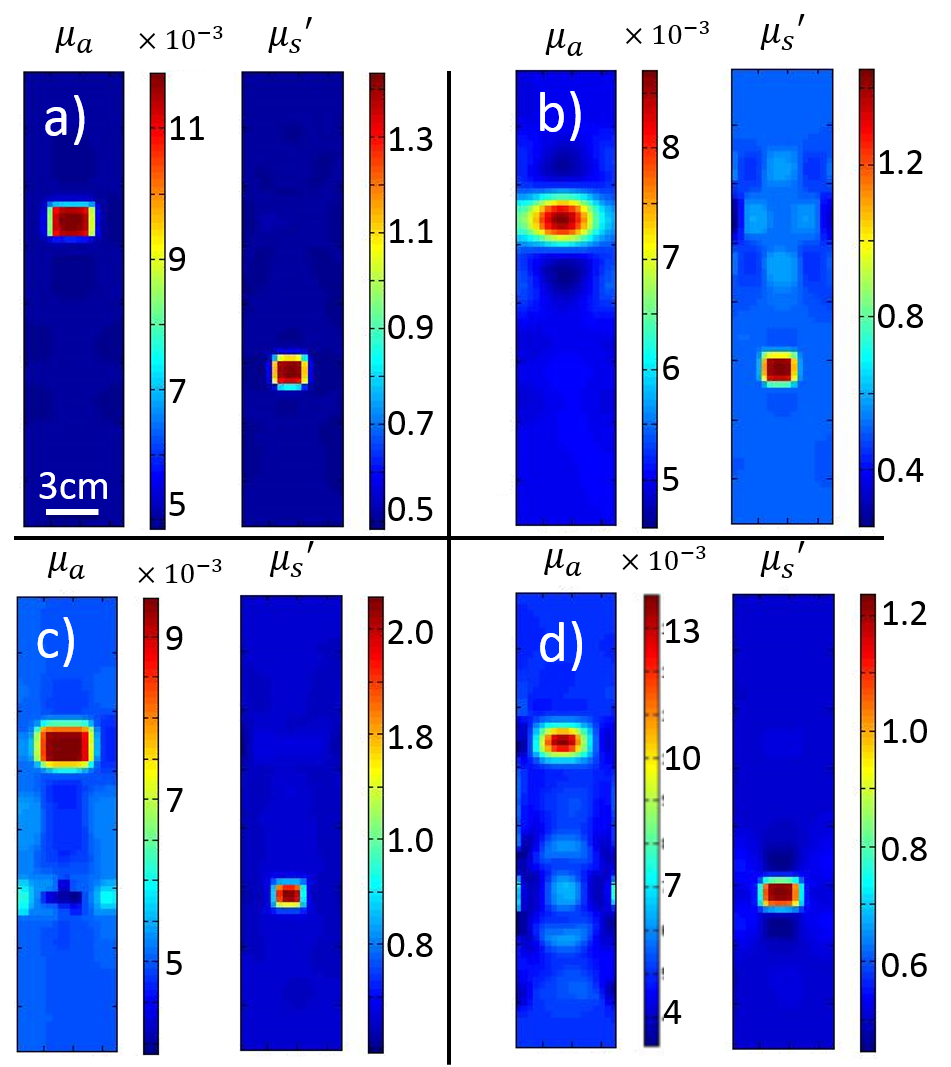
\includegraphics[width=12cm]{./figures/4_Gen3/2Dtvreg.png}
\caption[2D reconstructions for inclusions in Figure~\ref{fig:2Dsim}(a) with Total Variation (TV) regularization]{2D reconstructions for inclusions in Figure~\ref{fig:2Dsim}(a) but with Total Variation (TV) regularization. Values for $\Lambda$ the hyperparameter and $\beta$ the TV parameter for $\mua$ are varied separately. $\musp$: $\Lambda=1\times10^{-3}$, $\beta=1\times10^{-2}$ for all images. $\mua$: a)  $\Lambda=1\times10^{-2}$, $\beta=1\times10^{-3}$; b) $\Lambda=1\times10^{-3}$, $\beta=1\times10^{-1}$; c) $\Lambda=1\times10^{-2}$, $\beta=1\times10^{-3}$; d) $\Lambda=1\times10^{-4}$, $\beta=1\times10^{-3}$.}
\label{fig:2Dtvreg}
\end{center}
\end{figure}

Therefore, from our 2D reconstructions we learned that it can be useful to separately regularize absorption and scattering, and that it is important to optimize this regularization combination. Without this scheme, the reconstructed absorption spatial resolution (and contrast) is considerably worse than that of scattering. This effect was rationalized with the sensitivity curves, and an effort was made to find the independent regularization parameters for which the reconstructed $\mua$ and $\musp$ resolution was about the same. We will use these values, i.e., from 2D, in most of the other reconstructions (both simulations and experiment); ultimately, we will want to carry out a more comprehensive investigation of the independent regularization parameters for 3D simulated data and experimental reconstructions. Note, we also tried other regularization schemes (e.g., Tikhonov, PM), but we found that Total Variation (TV) regularization worked best, at least in the 2D simulations. Unfortunately, these additional degrees of freedom in regularization open up a great deal more phase-space for reconstruction optimization. On the other hand, and perhaps most importantly, we have discovered an important new avenue for image improvement!
%
\subsection{3D Reconstructions of Simulated Data}
Having explored different regularization schemes and parameter values in 2D simulations, we next moved to consider 3D simulations. Figure~\ref{fig:3Dsim} is a 3D reconstruction of two targets with the same diameter as in the 2D reconstructions and located in 3D within a $60$ mm thick slab. The top slices are closer to the source plane, and the lower slices are closer to the detector plane. The center slice at $30$ mm is shown. The sub-figures a) and b) are 3D reconstructions with uniform versus independent TV regularization. Figure~\ref{fig:3Dsim}(b) employs separate regularization for $\mua$, $\musp$, and we again see that the absorption spatial resolution and contrast improve. The gains exhibited in 3D thus appear to parallel our 2D results, and they reaffirm our expectation that improvements in 2D reconstructions translate to the 3D case. Of course, more work needs to be done to test whether the optimal regularization parameters are the same for 2D and 3D, but these initial results are encouraging.
\begin{figure}[t]
\begin{center}
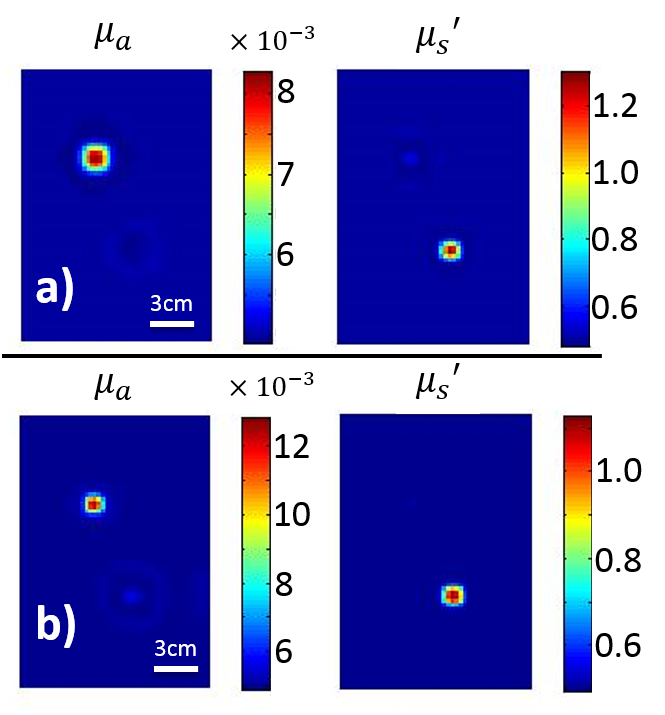
\includegraphics[width=10cm]{./figures/4_Gen3/3Dsim.png}
\caption[Simulated 3D reconstruction with TV regularization]{Simulated 3D reconstruction with TV regularization. a) $\mua,\musp$: $\Lambda=1\times10^{-4}$, $\beta=1\times10^{-2}$, b) $\mua$: $\Lambda=1\times10^{-4}$, $\beta=1\times10^{-2}$, $\musp$: $\Lambda=1\times10^{-3}$, $\beta=1\times10^{-2}$}
\label{fig:3Dsim}
\end{center}
\end{figure}
\begin{figure}[ph]
\begin{center}
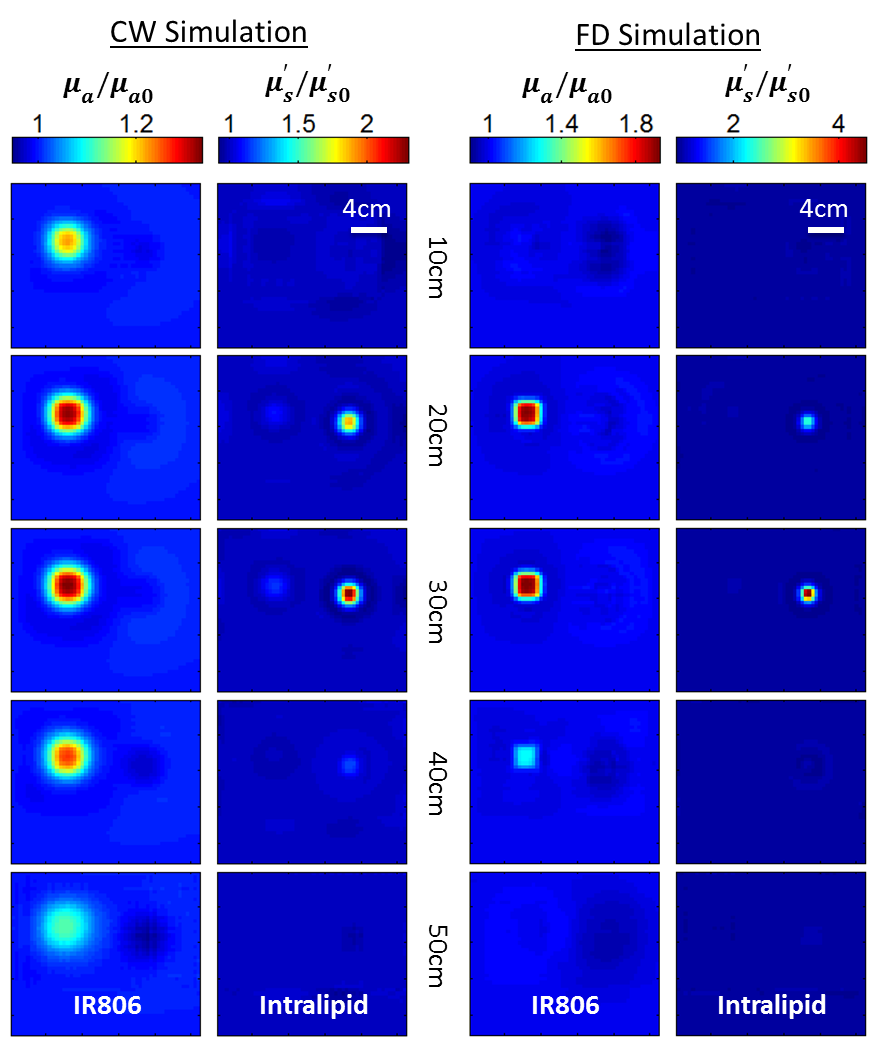
\includegraphics[width=14.5cm]{./figures/4_Gen3/3DsimFDCW.png}
\caption[Simulated 3D reconstructions of an absorption target (top left) and scattering target (bottom right) with CW and FD]{Simulation 3D reconstructions of an absorption target (top left) and scattering target (bottom right) with continuous-wave and frequency-domain data using TV regularization. The simulation shows that most of the crosstalk between absorption and scattering is mitigated with FD. The FD reconstruction of $\mua$ shows a 40\% contrast (($0.15~\rm{cm}^{-1}$ expected) with a 10\% crosstalk from $\musp$. The FD reconstruction of $\musp$ shows a 60\% contrast ($15~\rm{cm}^{-1}$ expected) at the scattering target with minimal crosstalk from the absorption target. Top slices are closer to the source plane and the lower slices are closer to the detector plane.}
\label{fig:3DsimFDCW}
\end{center}
\end{figure}
\begin{figure}[p]
\begin{center}
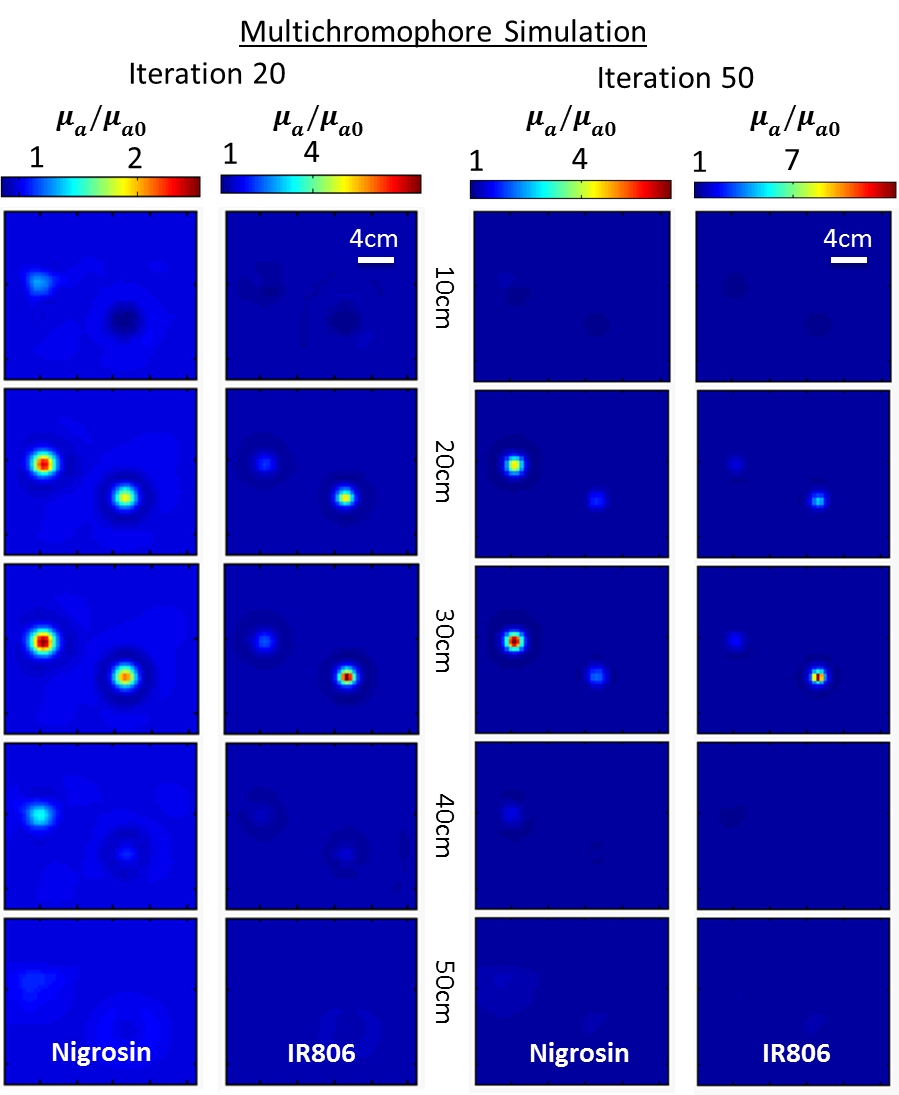
\includegraphics[width=14.5cm]{./figures/4_Gen3/3DsimMC.png}
\caption[Simulated 3D reconstruction of the two targets with different chromophores as shown in Figure~\ref{fig:2chromo}(b)]{Simulated 3D reconstruction of the two targets with different chromophores as shown in Figure~\ref{fig:2chromo}(b). The upper left target is filled with a Nigrosin contrast, and the bottom right target is filled with IR806 contrast. Each has an expected absorption that is twice the background Intralipid. The left columns show an early iteration wherein there is still crosstalk in the chromophores, but reasonable contrast. At late iterations the crosstalk is diminished, but the contrast is very high and the inclusion size small.}
\label{fig:3DsimMC}
\end{center}
\end{figure}

Figure~\ref{fig:3DFDCW} shows the simulated 3D reconstruction of two targets with a $3\times$ absorption (with spectrum corresponding to the dye IR806, upper left) and a $3\times$ scattering (corresponding to Intralipid, lower right) contrast. (Here we use targets in the simulations which are somewhat close to those in our 3D tissue phantom experiments.) For these reconstructions, the conjugate-gradient method was used with TV regularization. A CW reconstruction where only amplitude ($\Phi_{DC}$) information is used, and a FD reconstruction where both amplitude ($\Phi_{ac}$) and phase ($\theta$) data is used, are both shown in the figure. Slices are shown at $10~\rm{mm}$ intervals and are parallel to the source and detector planes. The slices stretch from the source plane (top) to the detector plane (bottom). The simulations clearly show, as expected, that without FD data (i.e., without amplitude and phase information), decoupling of $\mua$ and $\musp$ is poor. With FD data, importantly, most of this cross-talk is eliminated. Interestingly, even with noiseless data there is still some crosstalk from $\musp$ to $\mua$ ($10\%$ in this case) for our particular source-detector arrangement and geometry. Although the target medium inclusions are exactly in the slab center for both $\mua$ and $\musp$, there also seems to be a tendency for the reconstructed targets to be closer to the source plate. This shift might be caused by the sparse number of sources compared to the large number of detectors; in these simulations we have used just $60$ sources (selected symmetrically out of the $209$ total sources) and $209$ detectors to speed up our reconstructions for our analysis. This type of issue is something that we intend to explore more with further reconstructions.
\begin{figure}[t]
\centering
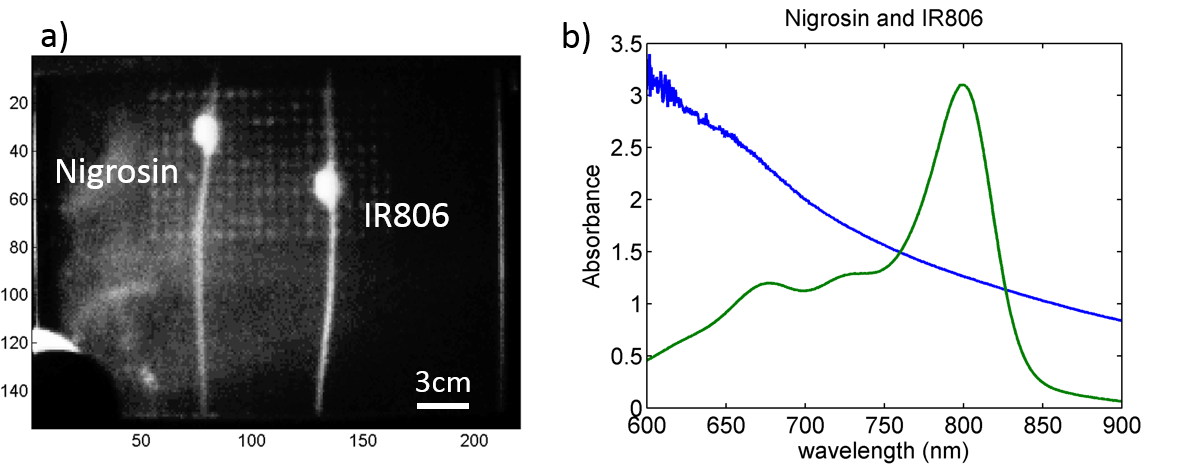
\includegraphics[width=13cm]{./figures/4_Gen3/2chromo.png}
\caption[Two targets used in multichromophore experiment and ink spectras]{a) Photograph of the two targets used in the multi-chromophore experiment; the images was taken by the Gen3 CCD. b) Spectra of the Nigrosin (blue) and IR806 (green) chromophores that were used in the multi-chromophore simulation and experiment.}
\label{fig:2chromo}
\end{figure}

Finally, we also ran a simulation of two target inclusions with different chromophores (but the same scattering); this reconstruction can in principle utilize spectral information. The contrast of the two dyes, Nigrosin and IR806, was again utilized to roughly match one of our tissue phantom experiments for which the spectral information is known (see Figure~\ref{fig:2chromo}). The simulation, in this case, shows how we can separate the two chromophores based on their spectral information. In the clinical case, of course, it is desirable to differentiate the chromophore concentrations of oxy- and deoxy-hemoglobin in tissue. Figure~\ref{fig:3DsimMC} shows the results at different iterations of the multi-chromophore reconstruction. Notice that at iteration 20, the reconstructed inclusions attain realistic values of the chromophore contrasts but there is still some crosstalk. At iteration 50, the chromophores are clearly differentiated spatially, but the contrast overshoots the expected values.  Again, more work is needed to clarify these observations and derive approaches to minimize the problems that surely could arise in real experiments.
%
\section{Tissue Phantoms}
After our work with simulations, we tested the Gen3 imager and reconstruction schemes with tissue phantoms that roughly mimic optical the properties and contrast of breast tissue. Hollow targets, $16~\rm{mm}$ in diameter (Figure~\ref{fig:targetpic}) with $1~\rm{mm}$ thick walls, were filled with optical contrast and submerged in a background solution.

Figure~\ref{fig:3DFDCW} shows the reconstruction using data from our Gen3 imager with the tissue phantoms. The background solution was mixed with India ink and Intralipid to have an approximate absorption and scattering of $\mua=0.05~\rm{cm}^{-1}$ and $\musp=5~\rm{cm}^{-1}$ at $785~\rm{nm}$. The targets were filled to have $3\times$ chromophore concentration (India ink, upper left) and $2\times$ scattering (Intralipid, lower right) relative to the background. The top slices are closer to the source plane and the lower slices are closer to the detector plane as in the 3D simulations.
\begin{figure}[!htp]
\begin{center}
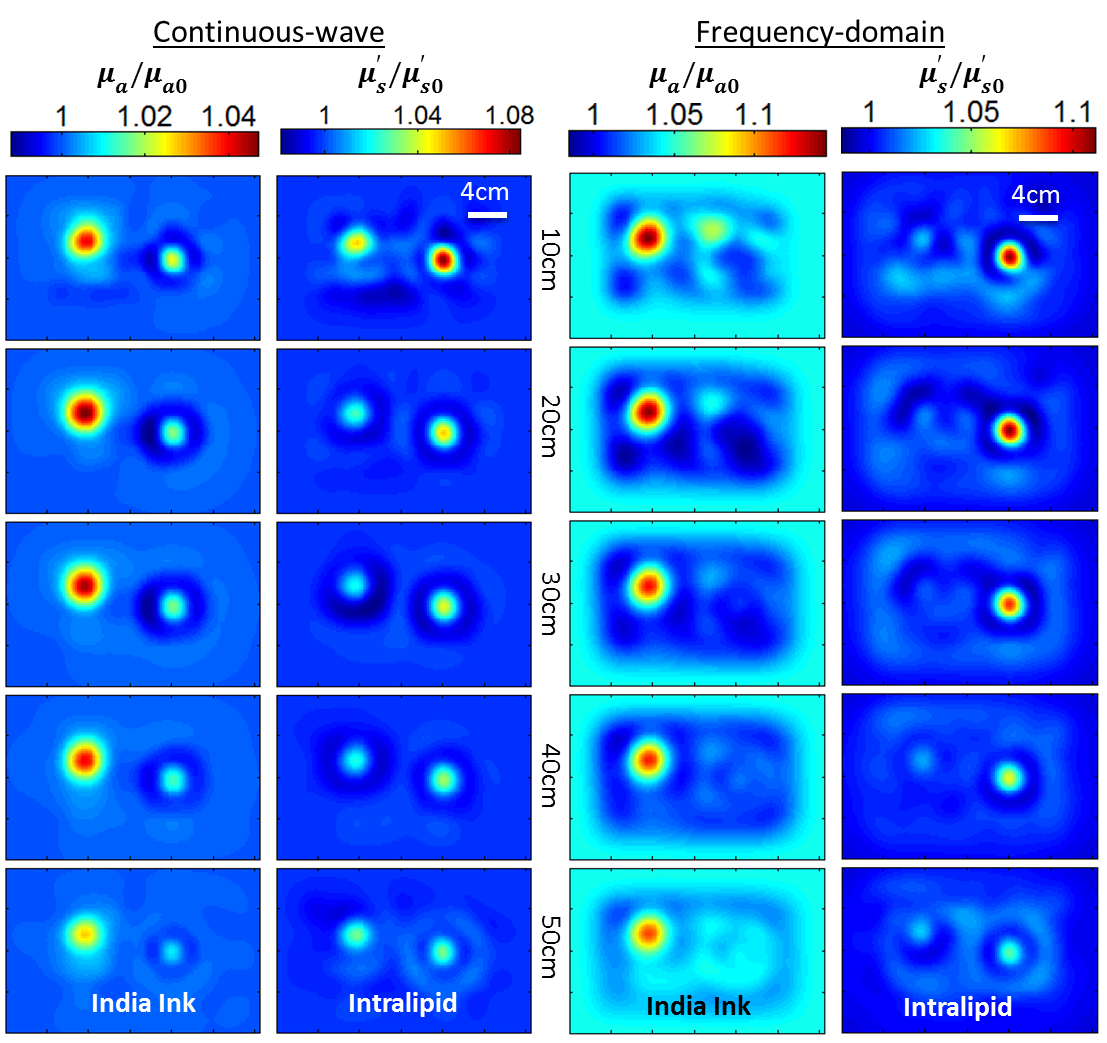
\includegraphics[width=14.5cm]{./figures/4_Gen3/3DFDCW.png}
\caption[3D reconstruction of tissue phantom in frequency-domain]{3D reconstruction of tissue phantom. The upper left target is India ink with $3\times~\mua$ contrast and the lower right target has a higher Intralipid concentration with $2\times~\musp$ contrast compared to the background. The CW reconstructions (left) have relatively low contrast and high crosstalk while the targets are well resolved spatially. In the FD reconstructions (right) noticeable artifacts near the source are apparent, but significantly less crosstalk between $\mua$ and $\musp$ is observed. The top slices are closer to the source plane and the lower slices are closer to the detector plane (as in the 3D simulations).}
\label{fig:3DFDCW}
\end{center}
\end{figure}

Again, as expected (but this time with experiment rather than simulation), we find that FD imaging reduces the crosstalk between absorption and scattering quite dramatically. There is a ``frame" of higher contrast levels on the edges of the absorption image in the FD reconstruction in Figure~\ref{fig:3DFDCW}, but that region lies outside the sensitivity range of our measurement and suggests that updated/better initial guesses of the background properties could improve our reconstruction. In addition, the image appears to suffer from artifacts near the source plane; these artifacts near the source and detector surfaces are known to arise in DOT, and methods exist that can be employed to ameliorate them, e.g., spatially variant regularization. However, we did not implement the spatially variant regularization technique here; it will be explored in future work. Nevertheless, the spatial structure of the reconstructed targets are well resolved in the transverse direction with some target broadening/elongation towards the source plate for both absorption and scattering objects. Again, a lower number of sources ($60$ of $209$) and detectors ($\sim320$ of $5000$ pixels) was utilized in the tomography so that we could carry out the reconstructions faster ($\sim6-8$ hours/reconstruction) with this data set. (Note, the small number of detectors is perhaps less of an issue than the sources, because adjacent pixels are averaged in software to increase the SNR.)

Although the spatial structure of the images is reasonably good, one nagging question concerns contrast (or lack thereof) of the tissue phantoms and to a lesser extent, contrast in our 3D simulations.  The actual reconstructed contrast is less than expected. This effect has been observed previously in DOT devices \cite{Pogue1997,McBride1999,Culver2003}, and it has largely been attributed to the spreading of the reconstruction contrast that arises when the target (in the reconstructed image) is spread out in size compared to the true target dimensions. The effective contrast in such images depends on a product of the target volume and target contrast (e.g., when a reconstructed absorption target is broadened in size (volume), then its absorption contrast is decreased in proportion to the volume). This problem is exacerbated in 3D, since there is an additional stretching in the longitudinal direction.  In addition, some of the underestimation of optical contrast is also due to systemic offsets inherent in the instrument or reconstruction method which can be compensated with calibration phantoms \cite{Jiang2003}. In fact, an area of research that these results suggest should be pursued, concerns how to rescale the image contrast; one approach to this problem is to utilize standard targets as part of every experimental run.
\floatbarrier
\begin{figure}[htp]
\centering
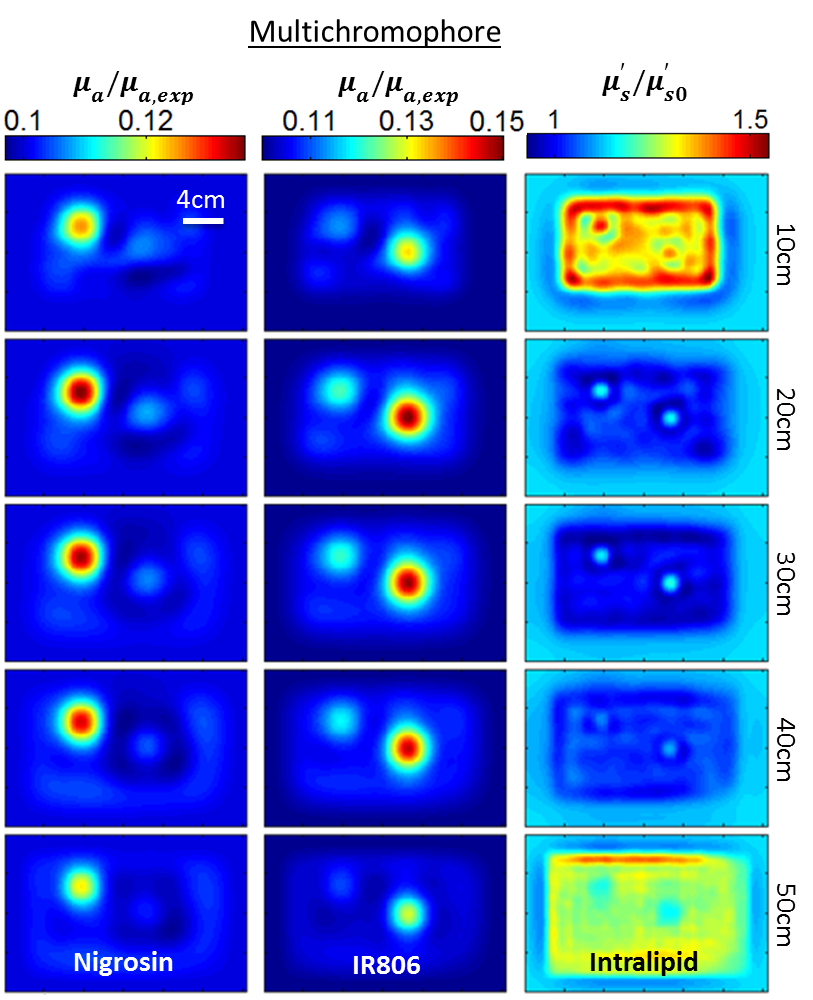
\includegraphics[width=11cm]{./figures/4_Gen3/3DMC.png}
\caption[3D reconstruction of the multi-chromophore data with Nigrosin (top left) and IR806 (bottom right) dyes with $2\times$ background absorption]{3D reconstruction of the multi-chromophore data with Nigrosin (top left) and IR806 (bottom right) dyes with $2\times$ background absorption. The absorption reconstructions looks similar to earlier iterations in the simulation (Figure~\ref{fig:3DsimMC}(a)). Increasing iterations past $\sim40$ for the data does not improve image quality as it is noise limited. Contrast level is low, but the main spatial features separate nicely.}
\label{fig:3DMC}
\end{figure}
In the case of our absorption and scattering targets, the integrated signal is $\Gamma =\delta \mua\cdot V$, where $\delta\mua$ is the fractional difference from the background, and $V$ is the target volume. Here we will use the approximate shape of the target object to estimate volume; using the FWHM to determine the bounding volume and integrating the $\delta\mua$ absorption within that volume, we determine $\Delta\Gamma^{\mua}=\Gamma_{recon}^{\mua}/\Gamma_{expected}^{\mua}=0.35$. This result (i.e., obtained by integration over the volume of the target object) is reasonable, especially given that our contrast is very large and will thus contribute to the signal in the nonlinear regime (i.e., outside of the small perturbing limit), and given that the object shapes are not perfect spheres, and given that our target objects have optical index of refraction differences with respect to the background that are not accounted for in the reconstructions. Similarly for the scattering contrast we found $\Delta\Gamma^{\musp}=0.36$. For comparison, in the CW case, we found $\Delta\Gamma^{CW,\musp}=0.16$ and $\Delta\Gamma^{CW,\musp}=0.05$. The resolution of the scattering target is quite good (except in the longitudinal direction as we have discovered with our simulations, but remember we do not employ any spatially variant regularization here). As expected the absorption targets are broader and larger than the scattering targets; in the future, we will explore more TV parameters to increase the absorption resolution.

In a different type of study, we employed two tissue phantoms to test the multi-spectral capabilities of the Gen3 imager. The two targets shown in Figure~\ref{fig:targetpic} were each filled with Nigrosin and IR806, respectively, to give approximately $2\times$ the absorption and the same scattering as the background Intralipid solution at $785~\rm{nm}$ ($\mua=0.04~\rm{cm}^{-1}$, $\musp=~8\rm{cm}^{-1}$). For this data set we increased the number of sources ($209$ of $209$), while keeping the number of detectors the same as the previous experiment ($\sim320$ of $5000$).

Figure~\ref{fig:3DMC} shows the 3D reconstruction of the two targets compared to the simulation. There is a clear separation of the chromophores in the image with a small amount of crosstalk, especially in the IR806 reconstruction ($\sim10\%$). Less crosstalk is apparent in the Nigrosin chromophore reconstruction, and this improvement could be due to the strong spectral sensitivity of the Nigrosin across the different wavelengths; by comparison, IR806 has very low contrast at the lower wavelengths. At higher iteration number, the simulations suggest that the two chromophores will eventually be differentiated. Unfortunately, at this time the data reconstruction is noise limited to 80 iterations after which no further improvements or difference in image quality can be found. For Nigrosin, $\Delta\Gamma^{Nigrosin} = 0.90$ which accounts for most of our contrast. The volume contrast for IR806 was also quite good with $\Delta\Gamma^{IR806} = 0.78$. The crosstalk in the scattering images from the absorbing targets were found to be $\sim10\%$ in this situation. Two reasons might explain the improve contrast: the increased number of sources could improve resolution and the lower perturbation ($2\times$ background instead of $\3times$) of the absorbers puts the problem more in the perturbative limit. Improving resolution with increased numbers of sources and detectors, improving our SNR which gives greater numbers of off-axis measurements, improving absorption resolution with different regularization, are all obvious issues we hope to explore in the near future with the Gen3 imager as a result of these experiments.
\floatbarrier
\section{Clinical Results: Breast Images}
The Gen3 breast imager resides the in Perelman Center for Advanced Medicine at the Hospital of the University of Pennsylvania. It is currently being tested on breast cancer patients. These first patient measurements have helped us to develop and improve the clinical hardware and software interfaces. Patient measurements present a unique set of challenges that constrain our data sets. The primary challenge is measurement time; we want to keep it as short as possible. Other challenges are present too. For example, the optical properties and breast boundary shapes vary quite a lot and are unique to each patient. In addition, unlike the tissue phantom experiments, the location and extent of the lesions in our clinical images are not known apiori; even if an MRI of the breast has been taken, the MRI measurement is usually made at a different time and in a different geometry, and of course, MRI has contrast mechanisms that are different from optics. Thus, with some trepidation, in this section we present first results from the study of two patients with the Gen3 breast imager.
%
\subsection{Patient Measurement Protocol}
First we describe the patient measurement protocol which was developed in accordance with the policies outlined by the University of Pennsylvania's Institutional Review Board (IRB). We have taken pains here to elucidate the protocol in a step-by-step manner. The future user of the instrument will benefit greatly from this step-by-step description.
\label{sec:protocol}
\begin{enumerate}[noitemsep]
\item Instrument setup and preparation.
\vspace{-2mm}
    \begin{enumerate}[noitemsep]
    \item The laser system, CCD, frequency generators, and all hardware are turned on and allowed to stabilize for at least 1 hour.
    \item A large polyethelene bag is placed within and then attached to the breast tank. Care is taken to insure that the bag is set flush against the source plate, window and side ports.
    \item The galvo switch alignment is adjusted to maximize light throughput and minimize instability before the measurement (note, this alignment can be done the night before).
    \item An optically matched India Ink and Intralipid solution is made before the patient arrives. A typical solution would have approximate absorption and scattering values of $\mua=0.06~\rm{cm}^{-1}$ and $\mua=8\rm{cm}^{-1}$, respectively, at 785nm.
    \end{enumerate}
\item Once the patient has been consented and instrument preparation has been made, the patient is placed on the Gen3 bed.
\vspace{-2mm}
    \begin{enumerate}[noitemsep]
    \item The breast is then softly compressed between the source and detector plate until the patient experiences only a slight discomfort. Typical plate separation is $6$ cm. When compression is complete, the plates are locked into place.
    \item The headrest and exam table height are adjusted for the patient. It is worthwhile to take the time needed for this adjustment to be sure the patient is comfortable. Patient comfort is important for reducing movement during the measurement.
    \end{enumerate}
\item The first data taken is associated with the profilometry measurements.
    \begin{enumerate}[noitemsep]
    \item Left side projector/camera measurement is taken.
    \item Then the right side projector/camera measurement is taken.
    \item Finally, the front illuminated Gen3 CCD measurement is made.
    \end{enumerate}
\item The breast imaging tank is filled with the India Ink and Intralipid solution that was prepared earlier (to match patient breast optical properties).
\item The system light intensity and the detection gain is adjusted to optimize detection dynamic range (Figure~\ref{fig:Clinical5}).
    \begin{enumerate}[noitemsep]
    \item The image intensifier MCP gain (typically 570V) is adjusted at brightest source position; this task enables us to check for signal saturation, etc.
    \item The attenuator is adjusted for pickoff light level to prevent detector saturation (i.e.,, to at most $\sim 50\rm{K}$ counts for brightest laser).
    \end{enumerate}
\item Start the breast DOT measurement. With the current instrumentation, the duration of this measurement is $\sim$35 minutes.
\item When the measurement is finished, then the patient will dress, and during this time period the tank is prepared for the reference measurement.
    \begin{enumerate}[noitemsep]
    \item At the same source plate and window separation (i.e., as used for the patient), fill the tank to top with Intralipid solution.
    \item Place the solid chest wall phantom on top of tank (Figure~\ref{fig:targets}, ensuring contact between phantom and Intralipid solution.
    \end{enumerate}
\item Begin reference measurement.
\item Obtain an image of the source positions. This image helps us locate the source positions in for the reconstruction.
    \begin{enumerate}[noitemsep]
    \item Empty breast imaging tank of Intralipid.
    \item Move source plate to detection plane.
    \item Illuminate fiber bundle face via the galvo, and take image of this source plate with the Gen3 CCD.
    \end{enumerate}
\item Calibrate Profilometry measurement using calibration target (Figure~\ref{fig:profcalib})
    \begin{enumerate}[noitemsep]
    \item Place calibration target in breast imaging tank.
    \item Left side projector/camera measurement.
    \item Right side projector/camera measurement.
    \end{enumerate}
\end{align}
%
\subsection{Cancer Patient #1}
Our first patient is a 79-year-old post-menopausal Caucasian female. Ultrasound found hypoechoic nodules which span approximately $18\times 10\rm{mm}$ at the 3:30 region of the breast, 4 cm from the areolar margin. A left breast core biopsy confirmed the presence of infiltrating mammary carcinoma with ductal and lobular features, and with intermediate grade nuclei. The patient consented to participate in our study in accordance with the consent policies outlined by the university's IRB. With the location of the tumor in mind, an effort was made to optimally place the patient's breast into the imaging tank. The plates were then compressed gently to fit the breast and achieve patient comfort. The final plate separation had a fixed distance of $64 \rm{mm}$.
\begin{figure}[bhtp]
\centering
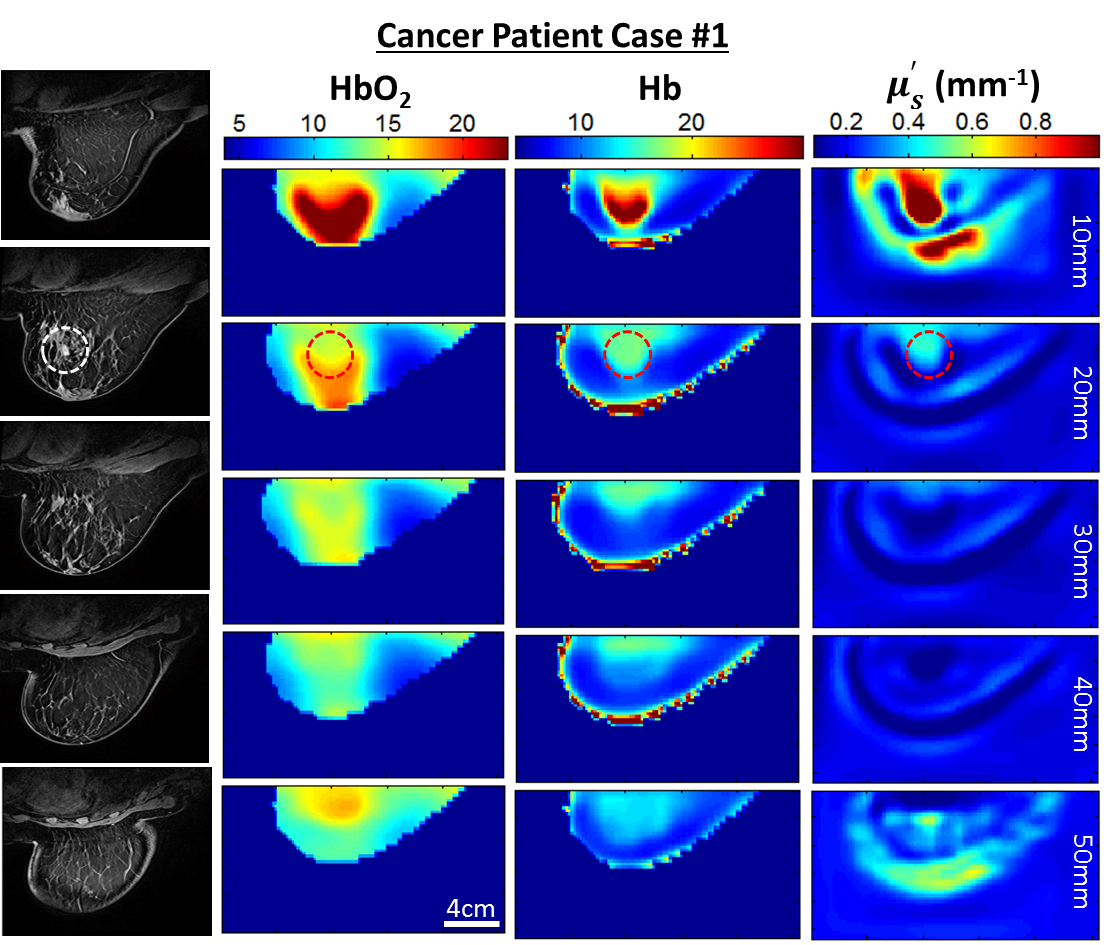
\includegraphics[width=14.5cm]{./figures/4_Gen3/G3096.png}
\caption[DOT images of $HbO_2$, $Hb$, and $\musp$: cancer patient #1]{MRI and DOT images of a 79-year-old post-menopausal Caucasian female with breast cancer. The first column shows an MRI of the cancer patient. Columns 2-4 show results from the 3D multi-spectral frequency-domain DOT reconstruction of  $HbO_2$, $Hb$, and $\musp$ at 785nm. The tumor location in the MRI is indicated by a white dotted circle. Red dotted circles indicate suspected tumor location on the DOT image. Note, however, the MRI and DOT breast compressions are similar but are not identical. Interesting features are apparent in both images with high $HbO_2$, $Hb$ and scattering near the tumor region (identified with biopsy clip in the MRI).}
\label{fig:G3096}
\end{figure}
\begin{figure}[htbp]
\centering
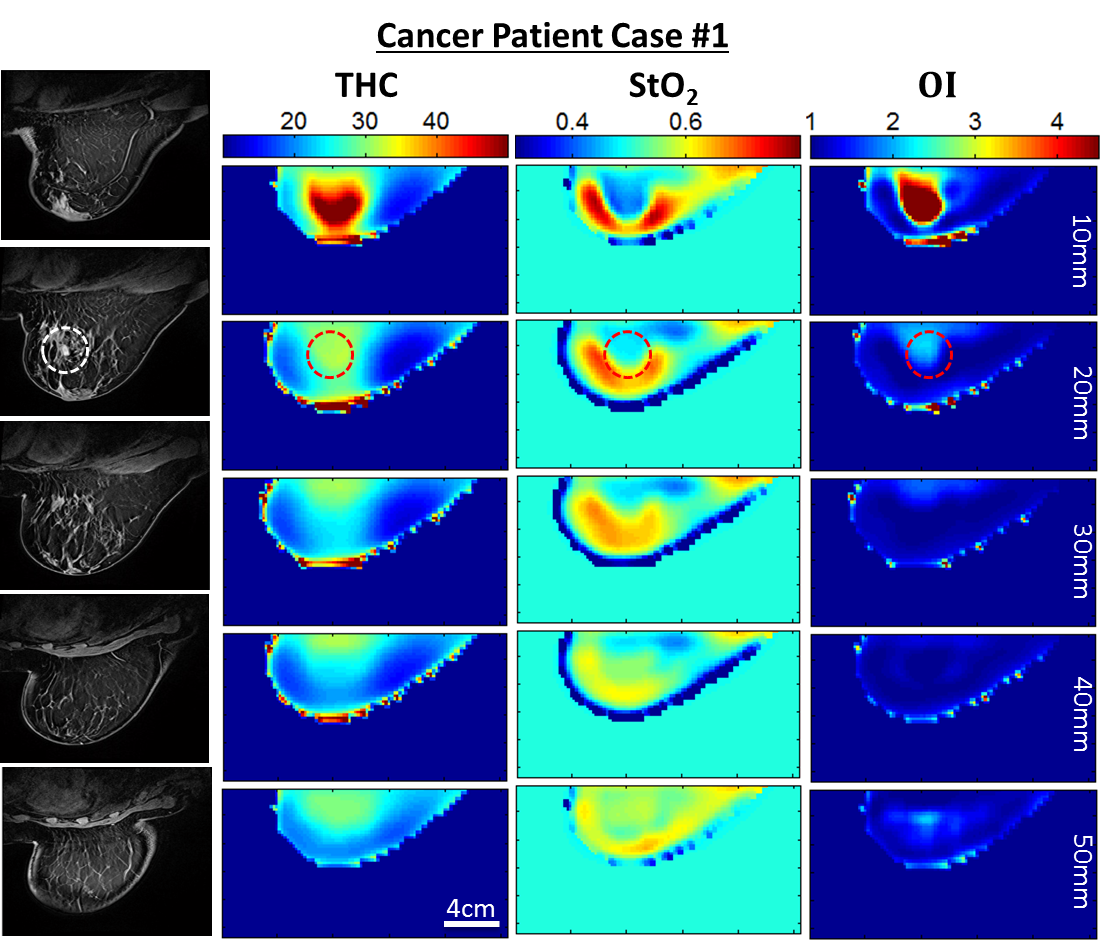
\includegraphics[width=14.5cm]{./figures/4_Gen3/G3096_2.png}
\caption[DOT images of $THC$, $StO_2$ and $OI$: cancer patient #1]{MRI and DOT images of a 79-year-old post-menopausal Caucasian female with breast cancer. The first column shows an MRI of the cancer patient. Columns 2-4 show results from the 3D multi-spectral frequency-domain DOT reconstruction of the $THC$, $StO_2$, and $OI$ at 785nm. The tumor location in the MRI is indicated by a white dotted circle. Red dotted circles indicate suspected tumor location on the DOT image. $StO_2$ shows depressed oxygenation region near the tumor location.}
\label{fig:G3096_2}
\end{figure}

The profilometry images were taken before the box was filled with Intralipid solution as described in Section~\ref{sec:protocol}. After optimization of the light level and detection gain for this particular breast, the DOT scan was initiated and run for 34 minutes. Finally, when the patient measurement was complete, a reference DOT scan was made with the box filled completely with Intralipid, and with the chest wall INO phantom (from Section \ref{sec:chestphant}, Chapter 3) placed over the breast tank hole. This block was placed on top of the tank in order to extend the diffuse medium in a manner analogous to the patient's chestwall; this configuration also helped prevent signal saturation caused by air boundaries. After the optical exam, the patient received a bilateral MRI. The MRI of the breasts was performed on a 1.5 Tesla magnet at HUP. In the lower-outer left breast, the MRI detected an area of abnormal enhancement that measured approximately $70\times 13\times 33~\rm{mm}$.

Figure~\ref{fig:G3096} shows the DOT reconstruction from the patient. T1 image slices from an MRI are shown, and the multi-spectral frequency-domain images of the hemoglobin concentration ($HbO_2$), the deoxy-hemoglobin ($Hb$), and scattering ($\musp$) are shown. The MRI slices was chosen to correspond to the slice of the DOT images by choosing equally spaced slices. In Figure~\ref{fig:G3096_2}, the derived parameters of total hemoglobin concentration $THC=HbO_2+Hb$, blood oxygen saturation $StO_2=HbO_2/THC$, and an optical index $OI=THC\times\musp/StO_2$ (normalized to healthy region) are exhibited. The optical index is a parameter which seeks to maximize optical contrast with the assumption that in tumors an elevated level of $THC$ and $\musp$ and depressed levels of $StO_2$ might be expected \cite{Tromberg2005,Cerussi2006,Choe2009}. There are significant artifacts in the $10~\rm{mm}$ plane, and we will explore different ways to suppress these artifacts as the research progresses. Moving inwards, away from the artifacts, the reconstructions exhibit physiological properties in expected range. In the 20mm slice, for example, the optical/physiological properties all fall within realistic values for the breast. Importantly, in the 20mm slice the DOT images show significant contrast for multiple optical parameters. The dotted red circle region where we suspect the tumor is located in Figure~\ref{fig:G3096}, show a contrast of $HbO_2\sim1.9$, $Hb\sim1.8$, $\musp\sim2.4$, $THC\sim1.7$, $StO_2\sim1$, and $OI\sim5.6$ when compared to the health region (i.e., as estimated from MRI and from other examinations). From the $Hb$ and $Hb$ images on the same plane the tumor can be estimated to be $25-35~\rm{mm}$ in diameter.

Much work remains. As in the simulations and phantom experiments, it appears that the tumor region is closer to the source plane than expected from the MRI. This first patient result is promising.  A tumor was imaged. This tumor was quite large, and it is certainly possible that the surrounding tissues also have optical properties that are different from normal tissues and therefore give rise to a further broadened spatial contrast. Furthermore, the imaging geometries of MRI and DOT are not the same, and thus the lesions could be spatially shifted in corresponding images. Of course, numerous issues remain to be addressed. For example, why does the contrast seem to be stronger near the source plane? We know that artifacts tend to arise near the source and detection planes, but we need to find ways to reduce these effects. In the future (see Chapter 5), many improvements can be made which should lead to improvements in the DOT images.
\floatbarrier
\subsection{Cancer Patient #2}
The second patient is a 68-year-old post-menopausal Caucasian female. She is positive for invasive mammary carcinoma with ductal and lobular features with associated in-situ carcinoma, and with intermediate nuclear grade. Ultrasound evaluation of this region showed a $15~\rm{mm}$ mass with associated calcifications at the 12:00 region of the breast. A right breast core biopsy confirmed the presence of invasive mammary carcinoma with ductal and lobular features associated with the in-situ carcinoma, and intermediate nuclear grade. This patient was consented in accordance with the policies outlined by Penn's IRB.
\begin{figure}[t]
\centering
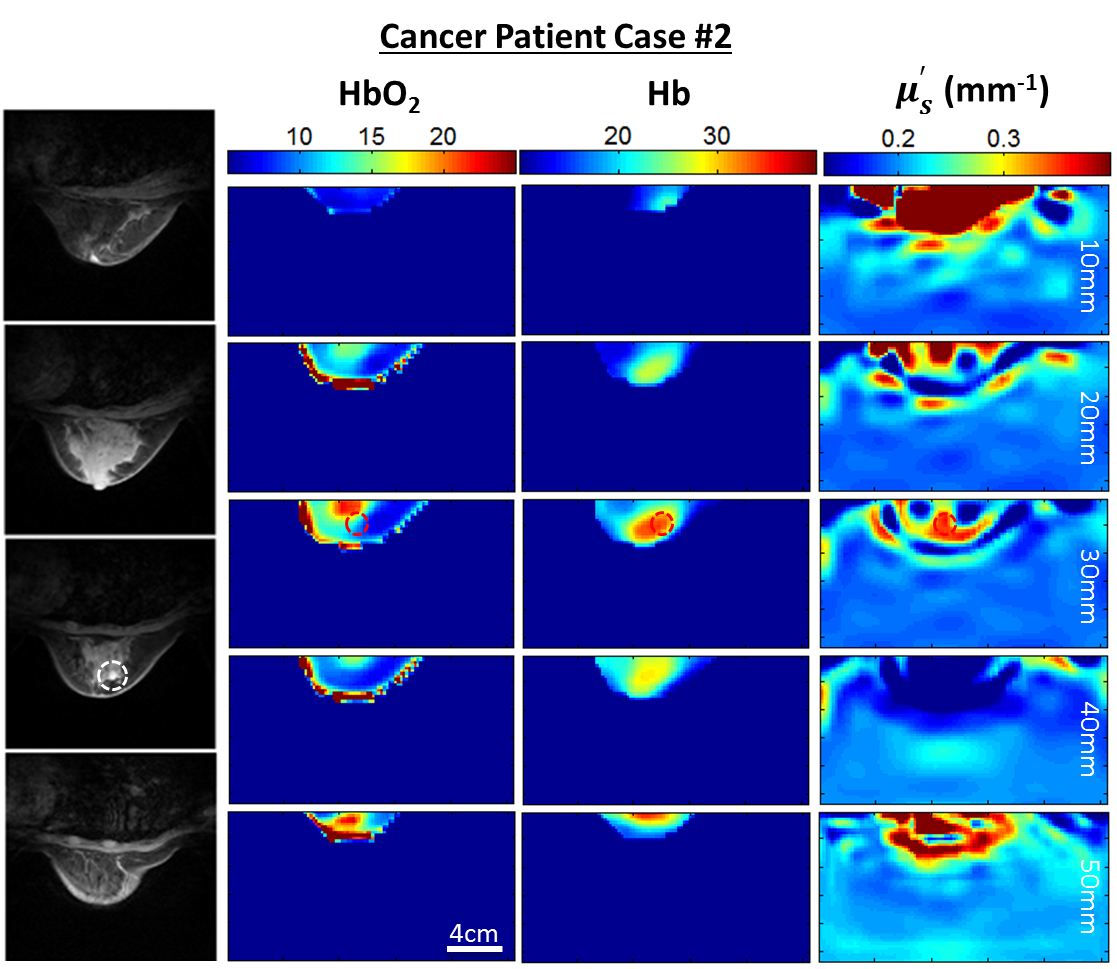
\includegraphics[width=14.5cm]{./figures/4_Gen3/G3098.png}
\caption[DOT images of $HbO_2$, $Hb$, and $\musp$: cancer patient #2]{MRI and DOT images of a  68-year-old post-menopausal Caucasian female with breast cancer. The first column shows the MRI of the cancer patient. Columns 2-4 show results from the 3D multi-spectral frequency-domain DOT reconstruction of the $HbO_2$, $Hb$, and $\musp$ at 785nm. The tumor location in the MRI is indicated by a white dotted circle. The MRI and DOT breast compressions are similar but are not identical. Possible tumor location shown in $HbO_2$ (identified with biopsy clip in the MRI). The $\musp$ image seem to have difficulty with this particular patient where there are large artifacts near the source plane.}
\label{fig:G3098}
\end{figure}
\begin{figure}[hbtp]
\centering
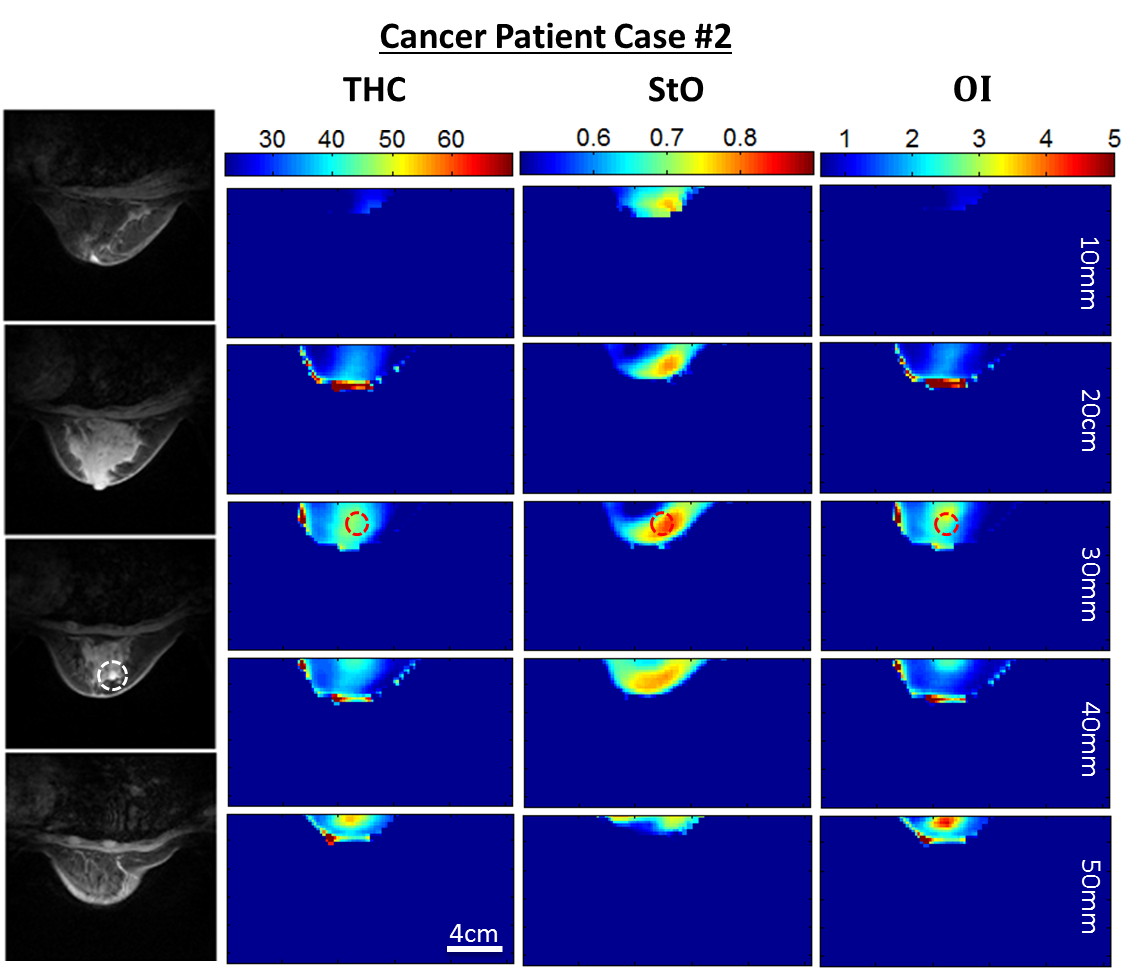
\includegraphics[width=14.5cm]{./figures/4_Gen3/G3098_2.png}
\caption[DOT images of $THC$, $StO_2$ and $OI$: cancer patient #2]{MRI and DOT images of a  68-year-old post-menopausal Caucasian female with breast cancer. The first column shows the MRI of the cancer patient. Columns 2-4 show results from the 3D multi-spectral frequency-domain DOT reconstruction of the $THC$, $StO_2$, and $OI$ at 785nm. Interesting features are apparent in both images with high $THC$, $StO_2$ and scattering near the tumor region.}
\label{fig:G3098_2}
\end{figure}
The individual's breast was gently compressed to achieve patient comfort; the plate separation was fixed distance at $60~\rm{mm}$. A measurement procedure similar to that of Patient #1 followed. After completion of the research study, the patient received an MRI bilateral image of her breasts in a 1.5 Tesla magnet. The MRI reported a moderate-to-large amount of glandular tissue. Approximately 9 mL of gadolinium contrast was administered intravenously for the MRI, and a 2 cm irregular mass was revealed in the upper-inner anterior right breast. There was also a linear enhancement in gadolinium contrast extending from the index mass anteriorly and posteriorly, with the overall extent of enhancement approximately $4~\rm{cm}$. In addition, a cluster of enhancing irregular masses was found in the upper outer breast at middle depth.

This patient presents a difficult case for x-ray, because of its high radiographic density. Figure~\ref{fig:G3098} and \ref{fig:G3098_2} shows the MRI as well as optical images for this patient. In this patient he tumor is difficult to locate but the suspected tumor has been circled in the $30~\rm{mm}$ slice of the DOT image. The dotted red circle region where we suspect the tumor is located show a contrast of $HbO_2\sim1.7$, $Hb\sim1.6$, $THC\sim1.4$, $StO_2\sim1.3$, and $OI\sim3$ when compared to the health region. The reconstruction algorithm also seemed to have difficulty with the scattering region, and thus it is challenging to ascertain a localized tumor area because of scattering artifacts near the source plane. As was the case with the first patient, the tumor in this case was quite large and somewhat diffuse, and it is certainly possible that the surrounding tissues also have optical properties that are different from normal tissues and therefore give rise to a further broadened spatial contrast; further, since the imaging geometries of MRI and DOT are not the same, the lesions in the corresponding images could be spatially shifted. Again, looking to the future (see Chapter 5), the first results show promise, but many improvements can and should be made which will very likely lead to improvements in the DOT images. 

\section{Summary}
In this chapter I have described a DOT breast imager that has been developed for clinical use. The instrument utilizes a spatially dense ($10^7$) source-detector pair arrangement, as well as multi-spectral and frequency-domain data types to push standalone DOT imaging capabilities in the clinical environment. These particular data types and source-detector geometry were explored with imaging simulations, and the instrument was characterized and validated with tissue phantoms. In addition, first image reconstructions from cancer patient data has been obtained. These steps represent a beginning and will soon lead to needed further development and optimization of image reconstruction and the hardware. Then the Gen3 imager will be translated to address specific clinical problems. 
